% letztes Update: 24-Dez-19
% letztes Update: 24-Dez-19 
\documentclass[a4paper,12pt,fleqn]{scrartcl}% 
\usepackage[margin=1in]{geometry}



% Metadaten einlesen
% letztes Update: 24-Dez-19 

% Eingabe der Metadaten

%-------Daten des Autors--------------------------
\newcommand{\autor}{Jan Unger}
\newcommand{\ort}{Wuppertal}
\newcommand{\website}{https://www.ju1.eu}

%-------Titel und Untertitel-----------------------
\newcommand{\titel}{dummy-notizenUbuntu-v03}% THEMA = TitelohneUmlaute
\newcommand{\untertitel}{~}% keinen Untertitel = ~
\newcommand{\typ}{Projekt}

%-------Datum: Jahr/Monat/Tag ---------------------
\newcommand{\version}{\date{2019/12/27 - Version: 669f69a}}% DATUM: alle Daten bitte in 8-stelliger Schreibweise angeben


%-deutsche Schlagwoerter(bitte getrennt durch Kommata auflisten)
\newcommand{\schlagwoerter}{PDF, Latex}

% Pakete
% <!-- update: 24-Nov-19 -->
\RequirePackage[l2tabu,orthodox]{nag}    % Detecting and warning about obsolete LaTeX commands
\RequirePackage[T1]{fontenc}      % Standard package for selecting font encodings
\RequirePackage{textcomp}         % LaTeX support for the Text Companion fonts
\RequirePackage[utf8]{inputenc}   % Accept different input encodings
\RequirePackage[dvipsnames,usenames]{xcolor}    % Driver-independent color extensions for LaTeX and pdfLaTeX

\RequirePackage[osf,sc]{mathpazo} % Fonts to typeset mathematics to match Palatino
\RequirePackage[scale=.9,semibold]{sourcecodepro}    % Use SourceCodePro with TeX(-alike) systems
\RequirePackage[osf]{sourcesanspro}    % Use SourceSansPro with TeX(-alike) systems

%\usepackage{lmodern}
%\usepackage{eulervm}
\usepackage[ngerman]{babel}% neuen deutschen Rechtschreibung
\usepackage[%
autostyle=true,% Anpassung an babelmain-
%english=american,%
german=guillemets% Design der deutschen Anfuehrungszeichen
]{csquotes}% praktische Anfuehrungszeichen

% bibliography
\usepackage[
bibencoding=utf8,
backend=bibtex,% bibtex, biber
sorting=nty,%Sortierung nach Name, Title, Year
style=alphabetic-verb,%beim Zitieren: alphabetic-verb, numeric, mla, science, phys, nature, ieee
%bibstyle=alphabetic%im Verzeichnis  : alphabetic, numeric, authoryear 
backref=false,backrefstyle=three+,url=true,urldate=comp,abbreviate=false,maxnames=20
]{biblatex} %Paket laden

\RequirePackage[dvipsnames,usenames]{xcolor}    % Driver-independent color extensions for LaTeX and pdfLaTeX

\RequirePackage{amsmath}          % AMS mathematical facilities for LaTeX
\RequirePackage{array}            % Extending the array and tabular environments
\RequirePackage{chngcntr}         % Change the resetting of counters


\RequirePackage{csquotes}         % Context sensitive quotation facilities
\RequirePackage{colortbl}         % Add colour to LaTeX tables
\RequirePackage{etoolbox}         % e-TeX tools for LaTeX
\RequirePackage{enumitem}         % Control layout of itemize, enumerate, description
\RequirePackage{float}            % Improved interface for floating objects
\RequirePackage{footnote}         % Improve on LaTeX's footnote handling
\RequirePackage{fnpct}\setfnpct{after-punct-space={-.2em}}    % Manage footnote marks’ interaction with punctuation
\RequirePackage{graphicx}         % Enhanced support for graphics
\RequirePackage{listings}         % Typeset source code listings using LaTeX

\RequirePackage{caption}          % Customising captions in floating environments
\RequirePackage{makeidx}          % Standard LaTeX package for creating indexes
\RequirePackage{multirow}         % Create tabular cells spanning multiple rows
\RequirePackage{scrhack}          % KOMA-Script File, contains improvement proposals for other packages
\RequirePackage[stretch=9,shrink=15,step=3,tracking=smallcaps,letterspace=75,final,babel=true]{microtype}    % Subliminal refinements towards typographical perfection
%\RequirePackage[osf,sc]{mathpazo} % Fonts to typeset mathematics to match Palatino
%\RequirePackage[scale=.9,semibold]{sourcecodepro}    % Use SourceCodePro with TeX(-alike) systems
%\RequirePackage[osf]{sourcesanspro}    % Use SourceSansPro with TeX(-alike) systems
\RequirePackage{textcase}         % Case conversion ignoring mathematics, etc
\RequirePackage{tikz}             % Create PostScript and PDF graphics in TeX
\RequirePackage{tocbasic}         % Management of tables/lists of contents (and the like)
\RequirePackage{todonotes}        % Marking things to do in a LaTeX document

\usepackage{calc}
\usepackage{setspace}

\usepackage{subcaption}

\usepackage{color}
\usepackage{multicol}
\usepackage{framed}
\usepackage[most]{tcolorbox}
\usepackage{wrapfig}

\usepackage{verbatim}
\usepackage{colortbl}
\usepackage{array, booktabs, caption}
\usepackage{makecell}
\usepackage{tcolorbox}
\usepackage{lipsum}
\usepackage{microtype}
\usepackage{pdfpages}% PDF Datei einbinden

% eigene Farbe definieren
\definecolor{farbe1}{gray}{0.5}
\definecolor{farbe2}{rgb}{1,0.4,0.3}
\definecolor{farbe3}{RGB}{255,60,40}
\definecolor{farbe4}{HTML}{FF00AA}
% Adobe Prozessfarben: CMYK: 100,50,0,35 -> 1,0.5,0,0.35
% Anwendung: \colorbox{blau}{Box}
\definecolor{blau}{cmyk}{1,0.5,0,0.35}     % 100,50,0,35
\definecolor{schwarz}{cmyk}{0.4,0.2,0.2,1} % 40,20,20,100
\definecolor{rot}{cmyk}{0,1,1,0.1}         % 0,100,100,10
\definecolor{orange}{cmyk}{0,0.55,0.61,0}     % 0,55,61,0
\definecolor{rot1}{cmyk}{0,0.95,0.31,0}       % 0,95,31,0
\definecolor{rot2}{cmyk}{0.13,1,0.4,0.04}     % 13,100,40,4
\definecolor{rot3}{cmyk}{0.29,1,0.47,0.34}  % 29,100,47,34
\definecolor{rot4}{cmyk}{0,0.95,0.9,0}        % 0,95,90,0
\definecolor{rot5}{cmyk}{0.22,1,1,0.19}   % 22,100,100,19
\definecolor{rot6}{cmyk}{0.33,1,0.95,0.05}   % 33,100,95,5
\definecolor{blau1}{cmyk}{0.71,0.15,0,0}      % 71,15,0,0
\definecolor{blau2}{cmyk}{0.85,0.42,0.18,0.04} % 85,42,18,4
\definecolor{blau3}{cmyk}{0.96,0.66,0.45,0.44}% 96,66,45,44
\definecolor{blau4}{cmyk}{0.83,0.56,0,0}      % 83,56,0,0
\definecolor{blau5}{cmyk}{1,0.77,0.1,0.01}  % 100,77,10,1
\definecolor{blau6}{cmyk}{1,0.86,0.4,0.35}  % 100,86,40,35
\definecolor{grau1}{cmyk}{0,0,0,0.2}          % 0,0,0,20
\definecolor{grau2}{cmyk}{0,0,0,0.4}          % 0,0,0,40
\definecolor{grau3}{cmyk}{0,0,0,0.8}          % 0,0,0,80
\definecolor{lila1}{cmyk}{0.36,0.67,0,0}      % 36,67,0,0
\definecolor{lila2}{cmyk}{0.45,0.8,0,0}       % 45,80,0,0
\definecolor{lila3}{cmyk}{0.73,1,0.26,0.17}   % 73,100,26,17
% hell - info
\definecolor{blau-hell}{cmyk}{0.25,0.13,0,0}     % 25,13,0,0
\definecolor{blau-dunkel}{cmyk}{0.75,0.45,0.05,0}   % 75,45,5,0
\definecolor{gruen-hell}{cmyk}{0.12,0,0.24,0}    % 12,0,24,0
\definecolor{gruen-dunkel}{cmyk}{0.48,0.09,0.8,0}  % 48,9,80,0
\definecolor{rot-hell}{cmyk}{0,0.26,0.14,0}      % 0,26,14,0
\definecolor{rot-dunkel}{cmyk}{0.19,0.8,0.66,0.08}    % 19,80,66,8
% hell Background
\definecolor{hell1}{cmyk}{0.74,0.04,0.28,0}       % C=74 M=4 Y=28 K=0
\definecolor{hell2}{cmyk}{0.42,0,0.03,0}          % C=42 M=0 Y=3 K=0
\definecolor{hell3}{cmyk}{0.12,0,0.38,0}          % C=12 M=0 Y=38 K=0
% dunkel Background
\definecolor{dunkel1}{cmyk}{0.96,0.59,0.59,0.71}  % C=96 M=59 Y=59 K=71
\definecolor{dunkel2}{cmyk}{0.97,0.73,0,0}        % C=97 M=73 Y=0 K=0
\definecolor{dunkel3}{cmyk}{0.07,1,1,0.2}         % C=7 M=100 Y=100 K=20  

\usepackage[
pdfstartview={FitV}, %Seite so hoch wie Fenster
pdffitwindow=true, %Fenster wird nicht
%automatisch an Seite angepasst
pdfcenterwindow=true, %mittiges Fenster
bookmarksnumbered=true
]{hyperref}

\usepackage{hyperxmp} % XMP-Daten fuer die PDF-Datei

%\hypersetup{%}

% pdf-Lesezeichen
\usepackage[%
openlevel=1, %am Beginn offen...
depth=3, %Tiefe der bookmarks insgesamt
numbered, %Kapitelnr bei bookmarks
]{bookmark}


%----------------------
% Marginalien
\newcommand{\marginlabel}[1]
{\mbox{}\marginpar{\RaggedRight\hspace{0pt}#1}}

\usepackage{nameref}

\usepackage{qrcode}% QR - Code Anwendung: \qrcode[hyperlink,height=4em]{\website}
% Hindergrundgrafik
\usepackage{wallpaper}
\usepackage{eso-pic}


\lstset{%
	basicstyle=\linespread{1}\ttfamily\small,
	floatplacement=htbp,
	captionpos=t,
	abovecaptionskip=.5\baselineskip,
	belowcaptionskip=.5\baselineskip,
	upquote=true,
	showstringspaces=false,
	inputencoding=utf8,
	tabsize=2,
	keywordstyle=\bfseries \color{black},
	commentstyle=\color{OliveGreen},
	stringstyle=\color{BurntOrange},
	breaklines=true,
	breakatwhitespace=true,
}

\lstset{literate={á}{{\'a}}1 {é}{{\'e}}1 {í}{{\'i}}1 {ó}{{\'o}}1 {ú}{{\'u}}1 {Á}{{\'A}}1 {É}{{\'E}}1 {Í}{{\'I}}1 {Ó}{{\'O}}1 {Ú}{{\'U}}1 {à}{{\`a}}1 {è}{{\`e}}1 {ì}{{\`i}}1 {ò}{{\`o}}1 {ù}{{\`u}}1 {À}{{\`A}}1 {È}{{\'E}}1 {Ì}{{\`I}}1 {Ò}{{\`O}}1 {Ù}{{\`U}}1 {ä}{{\"a}}1 {ë}{{\"e}}1 {ï}{{\"i}}1 {ö}{{\"o}}1 {ü}{{\"u}}1 {Ä}{{\"A}}1 {Ë}{{\"E}}1 {Ï}{{\"I}}1 {Ö}{{\"O}}1 {Ü}{{\"U}}1 {â}{{\^a}}1 {ê}{{\^e}}1 {î}{{\^i}}1 {ô}{{\^o}}1 {û}{{\^u}}1 {Â}{{\^A}}1 {Ê}{{\^E}}1 {Î}{{\^I}}1 {Ô}{{\^O}}1 {Û}{{\^U}}1 {œ}{{\oe}}1 {Œ}{{\OE}}1 {æ}{{\ae}}1 {Æ}{{\AE}}1 {ß}{{\ss}}1 {ű}{{\H{u}}}1 {Ű}{{\H{U}}}1 {ő}{{\H{o}}}1 {Ő}{{\H{O}}}1 {ç}{{\c c}}1 {Ç}{{\c C}}1 {ø}{{\o}}1 {å}{{\r a}}1 {Å}{{\r A}}1 {€}{{\EUR}}1 {£}{{\pounds}}1 {~}{{\textasciitilde}}1 {-}{{-}}1 }

% Abb., Tab., Quellcode
\renewcaptionname{ngerman}{\contentsname}{Inhalt}
\renewcaptionname{ngerman}{\listfigurename}{Abbildungen}
\renewcaptionname{ngerman}{\listtablename}{Tabellen}
\renewcaptionname{ngerman}{\figurename}{Abb.}
\renewcaptionname{ngerman}{\tablename}{Tab.}
% names
\let\defaultlstlistingname\lstlistingname\renewcommand\lstlistingname{\iflanguage{ngerman}{Quelltext}{\defaultlstlistingname}}

% captions
\addtokomafont{caption}{\small}
\addtokomafont{captionlabel}{\bfseries\sffamily\small}
\setcapindent{\parindent}


% list of contents
\setcounter{tocdepth}{3}
\setcounter{secnumdepth}{3}




\definecolor{mycolor}{rgb}{0.122, 0.435, 0.698}% Rule colour
\makeatletter
\newcommand{\mybox}[1]{%
	\setbox0=\hbox{#1}%
	\setlength{\@tempdima}{\dimexpr\wd0+13pt}%
	\begin{tcolorbox}[colframe=mycolor,boxrule=0.5pt,arc=4pt,
		left=6pt,right=6pt,top=6pt,bottom=6pt,boxsep=0pt,width=0.95\textwidth]
		#1
	\end{tcolorbox}
}
\makeatother

% Parts list tables
\renewcommand\theadfont{\bfseries}
\newcolumntype{I}{ >{\centering\arraybackslash} m{2cm} }  % part image
\newcolumntype{N}{ >{\centering\arraybackslash} m{2cm} }  % part name
\newcolumntype{Q}{ >{\centering\arraybackslash} m{1cm} }  % ref & menge

% tables
\newcolumntype{L}[1]{>{\raggedright\let\newline\\\arraybackslash\hspace{0cm}}m{#1}}
\newcolumntype{C}[1]{>{\centering\let\newline\\\arraybackslash\hspace{0cm}}m{#1}}
\newcolumntype{R}[1]{>{\raggedleft\let\newline\\\arraybackslash\hspace{0cm}}m{#1}}
\captionsetup[table]{belowskip=.5\baselineskip,aboveskip=.5\baselineskip}

\newcommand\partimg{\includegraphics[width=2cm,height=1.25cm,keepaspectratio]}


\usepackage{blindtext}% \blindtext
% Erzeugung mehrseitiger Tabellen
\usepackage{longtable}

% Eigene Befehle können hier definiert werden
%% Textauszeichnung
% \emph{kursiv}
% \textrm{Antiqua}, \textsf{Grotesk}, \texttt{Maschinenschrift},
% \textmd{normal}, \textbf{breiter}, \textup{aufrecht}, \textsl{geneigt},
% \textit{kursiv}, \textsc{Kapitaelchen}

%% Schriftgroesse
% \tiny{winzig}, \scriptsize{sehr klein}, \footnotesize{klein},
% \small{klein}, \normalsize{normal}, \large{gross}, \Large{groesser},
% \LARGE{ganz gross}, \huge{riesig}, \Huge{gigantisch}

%% eigene Befehle definieren
% Textauszeichnung: \wort{Beispiel}, \fremdwort{prezioes}
\newcommand{\wort}[1]{\emph{#1}}
\newcommand{\fremdwort}[1]{\textsf{#1}}

%% Textabstand:  Verwendung: \abstand{}
\newcommand{\abstand}[1]{\hspace{10em}{#1}}
%% quad, qquad, hspace{10em}, vspace{10em}
%
% Wichtig (Optionale Parameter)
%% Wort Kursiv u. in Farbe
\newcommand{\wichtig}[2][rot6]{\textcolor{#1}{\emph{#2}}}

% Literatur laden
\bibliography{content/literatur}%


% Artikel
\usepackage{fancyhdr}
\pagestyle{fancy}
\lfoot{\textbf{\titel}}% Thema
\rfoot{Seite \thepage}% Seite
\lhead{\textbf{\leftmark}}
\rhead{\textbf{\rightmark}}
\cfoot{}
\renewcommand{\footrulewidth}{0.8pt}
\renewcommand{\headrulewidth}{0.8pt}
\doublespacing
\setlength{\parindent}{1cm}

%% Kapitelueberschriften farbig
\usepackage{sectsty}
\chapterfont{\color{rot6}}
\sectionfont{\color{rot6}}
\subsectionfont{\color{rot6}}
\subsubsectionfont{\color{rot6}}

% PDF/A-1b-Konformitaet Optionen wichtig!
%		pdftitle, pdfauthor, pdfsubject, pdfkeywords, pdfa	
\hypersetup{% Setup fuer PDF-/Hypertext-Generierung + Metadaten
	pdftitle={\titel},
	pdfauthor={\autor},
	pdfsubject={\typ},
	pdfkeywords={\schlagwoerter},
	pdflang=de,
	bookmarks=true,
	pdfdisplaydoctitle=true,
	colorlinks=true,
	plainpages=false,
	%allcolors=black,
	colorlinks=true,	   
	linkcolor=blau5,		
	filecolor=black,		
	urlcolor=blau5,			
	citecolor=black,	
	hypertexnames=false,
	pdfpagelabels=true,
	hyperindex=true,
	unicode=true,
	pdfcaptionwriter={\autor},
	pdfcontactcity={\ort},
	pdfcontactcountry={Deutschland},
	pdfcontactregion={NRW},
	pdfcontacturl={\website},
	pdfmetalang={de},
	pdftex=true,             % bitte nicht aendern!
	hypertexnames=false,     % bitte nicht aendern!
	pdfa=true,  % bitte nicht aendern! NEU: PDF/A-flag
	breaklinks=true,%
	bookmarksnumbered=true,
	breaklinks=true
}

\begin{document}
\title{\titel}% Thema
\author{\autor}
%\date{\today}
\date{2019/10/20}

%\maketitle
%\tableofcontents

%---------------------
	%% letztes Update: 20-Okt-19
\section{\LaTeX}
\label{latex}

\subsection{Zitieren}
\label{zitieren}

Literaturlistenverwaltungsprogramm: JabRef 

%\nocite{*} Auch unzitierte Literatur wird gedruckt

Zitat: vgl. \cite{monk_action_buch:2016} u. \cite{kofler_linux:2017} 

\subsection{Quellcode}
\label{quellcode}

Hallo Welt (vgl. Quellcode \ref{hallo_welt}).
\begin{lstlisting}[caption={Hallo Welt},label={hallo_welt},language=C++% C, TeX, Bash, Python
]%--Code einfügen--%

#include <iostream>
int main(){
	std::cout << "Hallo Welt!" << std::endl;
}
\end{lstlisting}

hallowelt.cpp (vgl. Quellcode \ref{hallo_welt_ex}).
\lstinputlisting[caption={hallowelt.cpp},label={hallo_welt_ex},language=C++% C, TeX, Bash, Python
]{content/bsp/hallowelt.cpp}

\LaTeX -Syntax (vgl. Quellcode \ref{latex_syntax}). 
\begin{lstlisting}[caption={\LaTeX-Syntax},label={latex_syntax},language=TeX% C, TeX, Bash, Python
]%--Code einfügen--%

\subsection{Quellcode}
\label{quellcode}
\end{lstlisting}


\subsection{Text und Absatz}
\label{text_absatz}
Damit Ihr indess erkennt, woher dieser ganze Irrthum gekommen ist, und weshalb man die Lust anklagt und den Schmerz lobet, so will ich Euch Alles eröffnen und auseinander setzen, was jener Begründer der Wahrheit und gleichsam Baumeister des glücklichen Lebens  vornehmen, wenn er nicht einen Vortheil davon erwartete. Wer dürfte aber wohl Den tadeln, der nach einer Lust verlangt, welcher keine Unannehmlichkeit folgt, oder der einem Schmerze ausweicht, aus dem keine Lust hervorgeht?

Dagegen tadelt und hasst man mit Recht Den, welcher sich durch die Lockungen einer gegenwärtigen Lust erweichen und verführen lässt, ohne in seiner blinden Begierde zu sehen, welche Schmerzen und Unannehmlichkeiten seiner deshalb warten. Gleiche Schuld  von sich weisen darf. Deshalb trifft der Weise dann eine Auswahl, damit er durch Zurückweisung einer Lust dafür eine grössere erlange oder durch Uebernahme gewisser Schmerzen sich grössere erspare. 

\noindent Deshalb trifft der Weise dann eine Auswahl, damit er durch Zurückweisung einer Lust dafür eine grössere erlange oder durch Uebernahme gewisser Schmerzen sich grössere erspare. 

\subsection{Listen}
\label{listen}
\begin{enumerate}
	\item Beschreibung
	\item Bild
	
	\begin{figure}[H]
 		\centering
		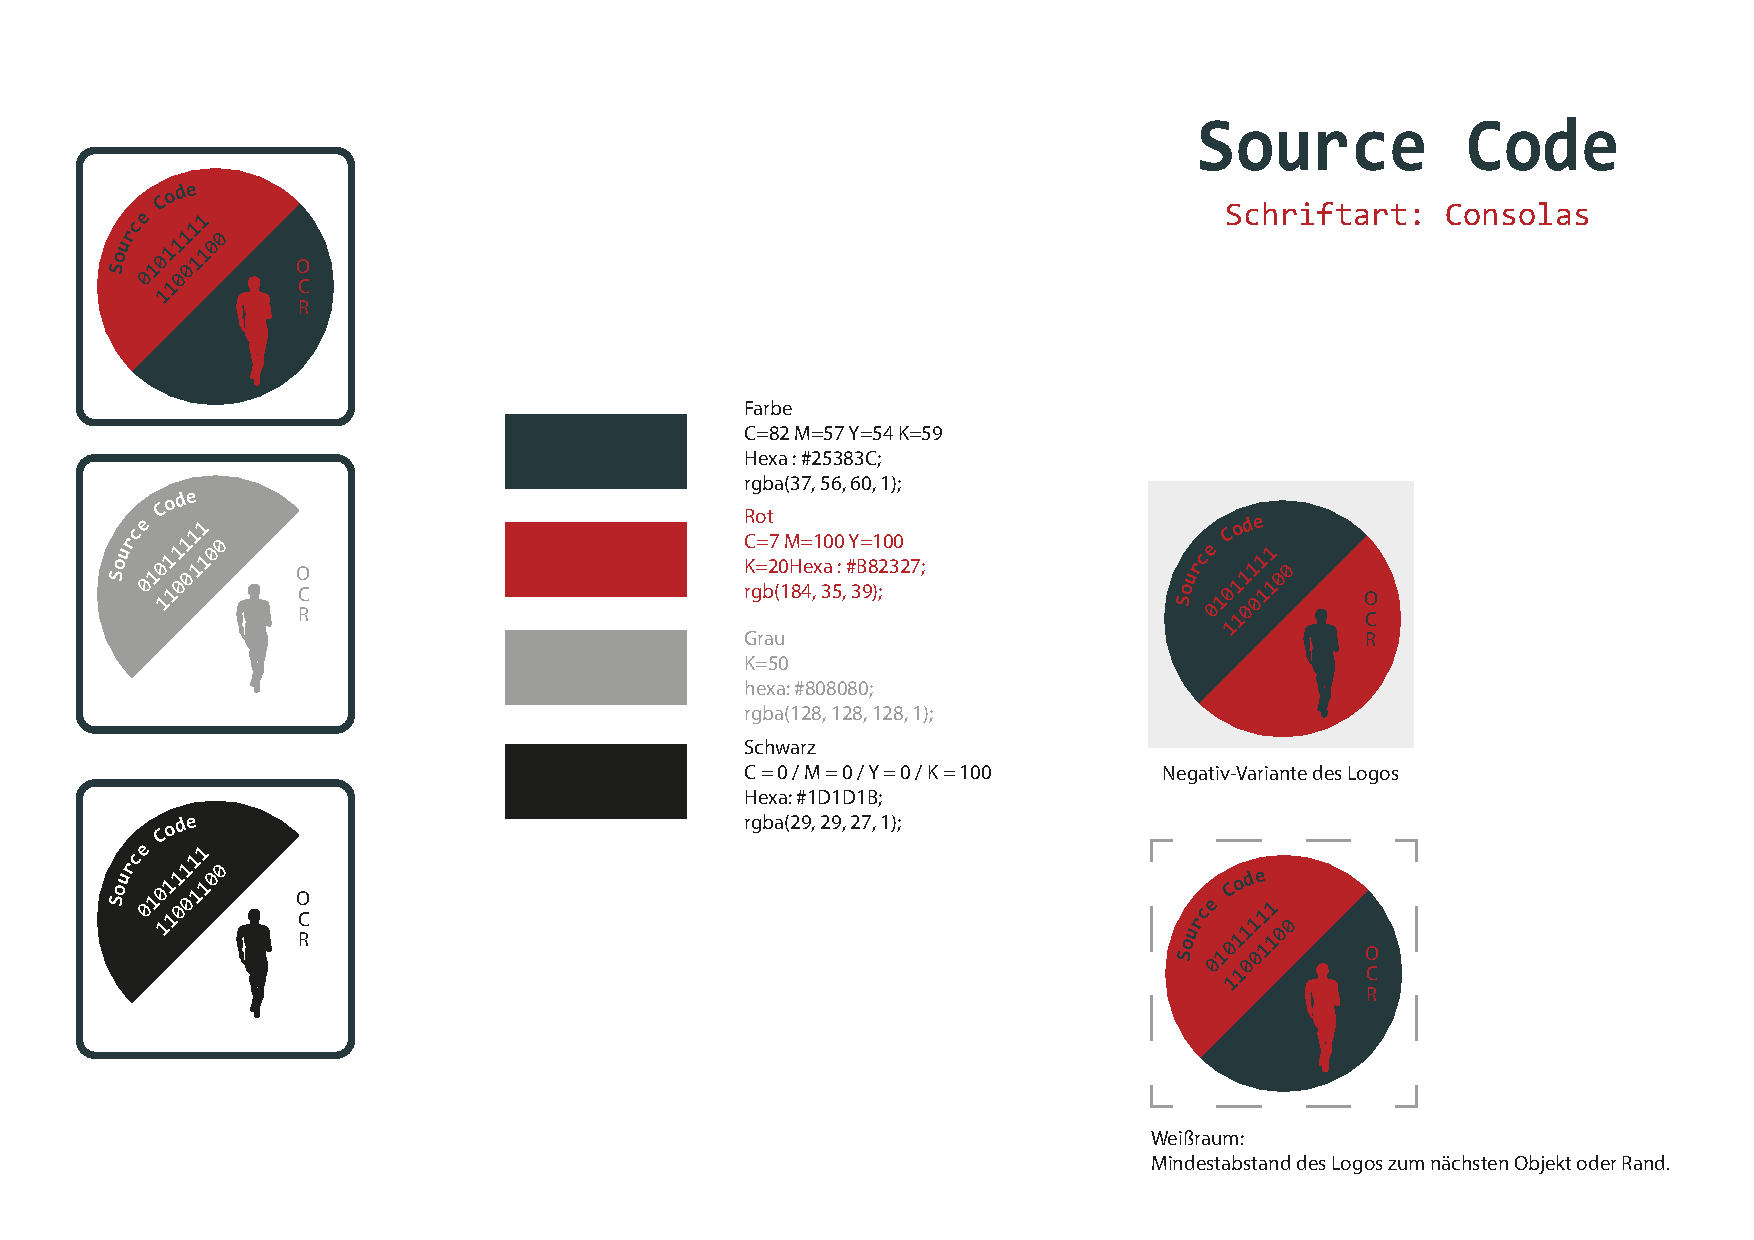
\includegraphics[width=.55\textwidth]{content/bsp/Logo-Details.pdf}
	\end{figure}

	\item Tabelle
	\newline 
	
	\begin{centering}
		\begin{tabular}[3] {| l | l | l |}
			\hline
			\textbf{Control Board Label} & \textbf{Wire Color} & \textbf{Signal} \\ \hline
			VCC & Red & Motor + \\ \hline
			GND & Black & GND \\ \hline
		\end{tabular} 	
	\end{centering}

	\item Werte

	\begin{itemize}
		\item \textbf{Temperature1:} ~ 30
		\item \textbf{M1/M2 Amps:} ~ 0.00
	\end{itemize}

\end{enumerate}

\begin{enumerate}
	\item Aufzählung
	\item Aufzählung
	\item Clone the code repo:
	\begin{enumerate}
		\item git clone https://github.com/ju-bw/notizenDummyWin10-v03.git 
		\item git checkout master
		\item git pull
	\end{enumerate}
\end{enumerate}

\begin{itemize}
	\item Punkt
	\item Punkt
\end{itemize}

\begin{enumerate}
	\item[] Direct downloadable Raspbian Buster image: 
	\item[] \href{https://downloads.raspberrypi.org/raspbian/images/raspbian-2019-07-12/2019-07-10-raspbian-buster.zip}{https://downloads.raspberrypi.org/raspbian/images/raspbian-2019-07-12/2019-07-10-raspbian-buster.zip}
\end{enumerate}


\subsection{Referenz und Links}
\label{referenz_links}

\begin{itemize}
	\item Link \href{https://www.ju1.eu/}{https://www.ju1.eu/}.
	\item \href{https://www.ju1.eu/}{Website}.
	\item File (siehe \href{https://github.com/ju-bw/dummy-Notiz-Win10-v03/Readme.pdf}{/Readme.pdf})
	\item Bild (siehe Abb. \ref{bild})
	\item Tabelle (siehe Tab. \ref{komponenten})
	\item Kapitel (siehe Kap. \ref{latex})
	\item Textfußnote \footnote{Fußnote}.
\end{itemize}


\subsection{Bilder}
\label{bilder}

%Bild (siehe Abb. \ref{bild})
\begin{figure}[H]
	\centering
	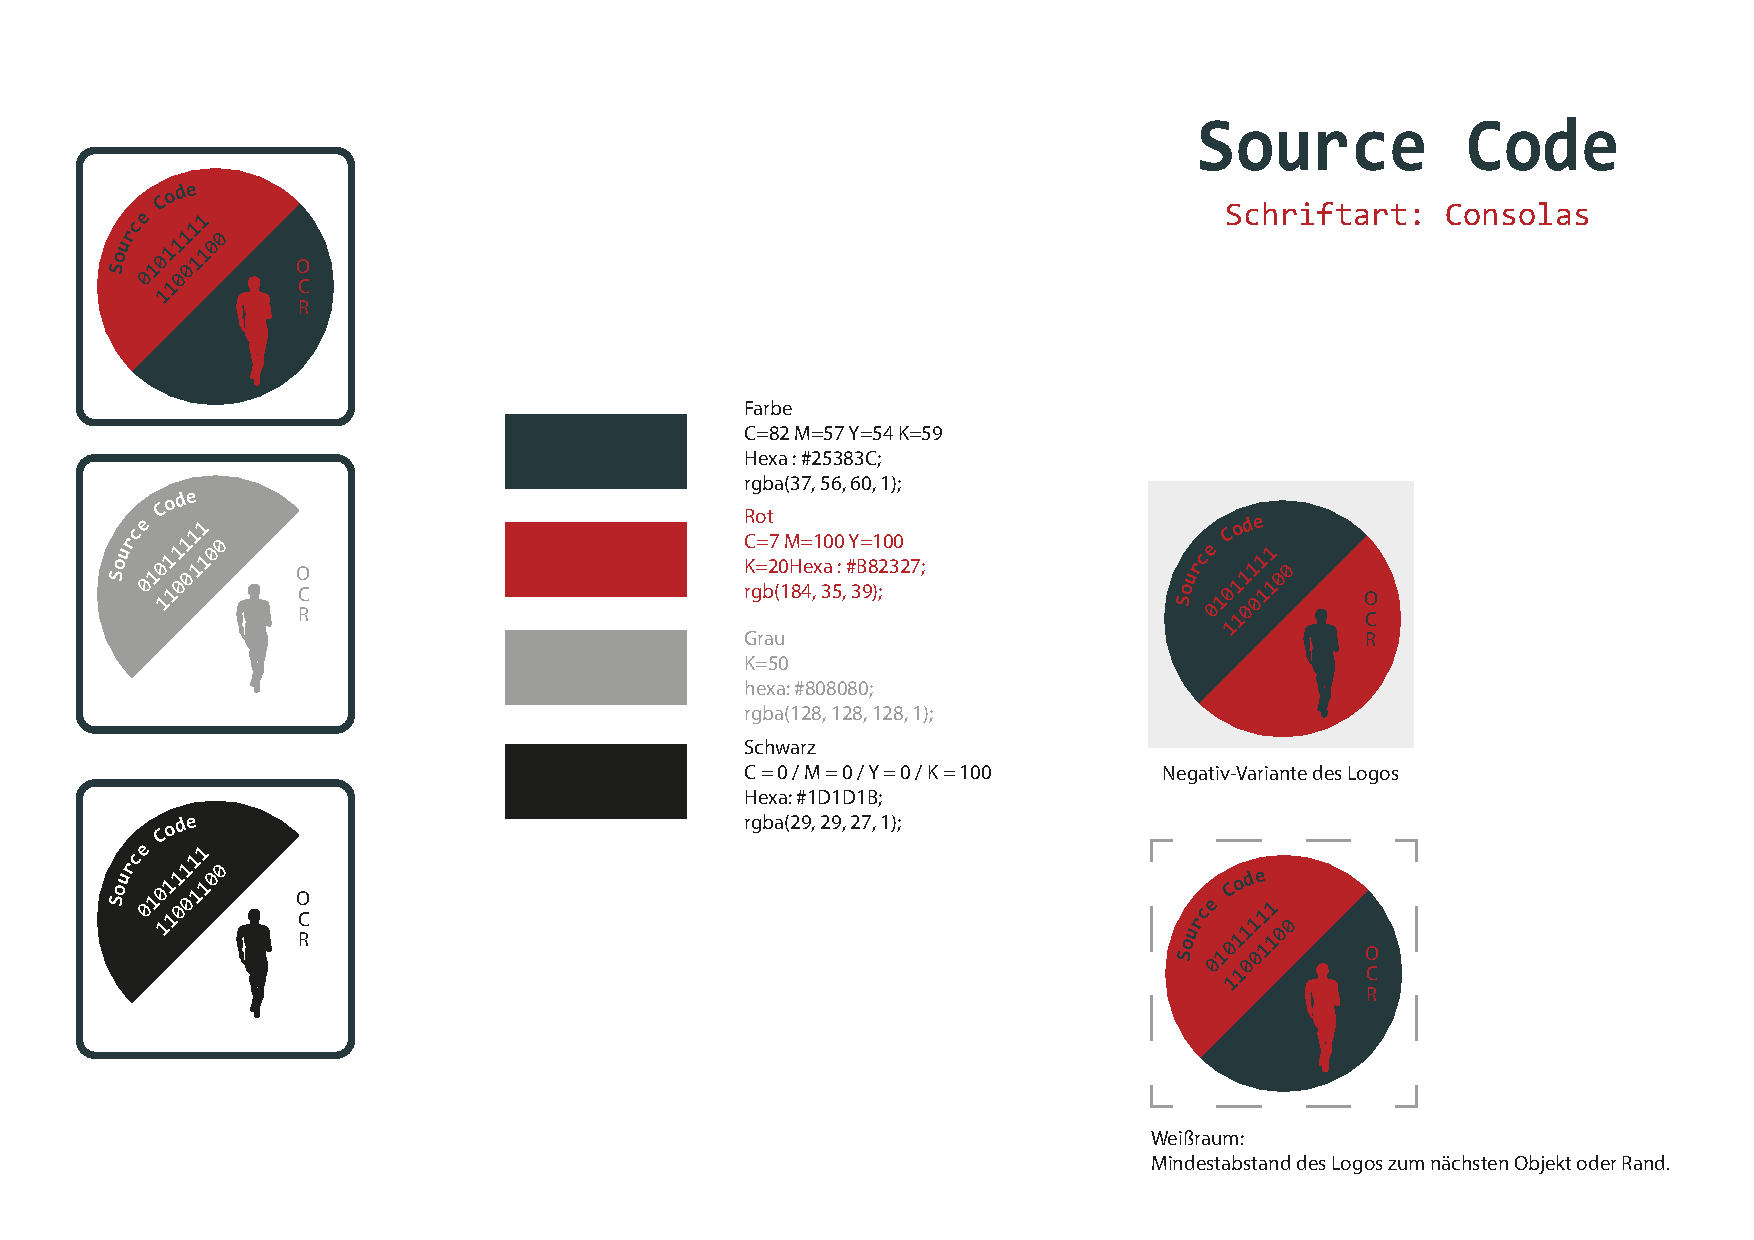
\includegraphics[width=.55\textwidth]{content/bsp/Logo-Details.pdf}
	%---------------------------------
	\caption{Bild} \label{bild}
\end{figure}

\begin{figure}[H]
	\centering
	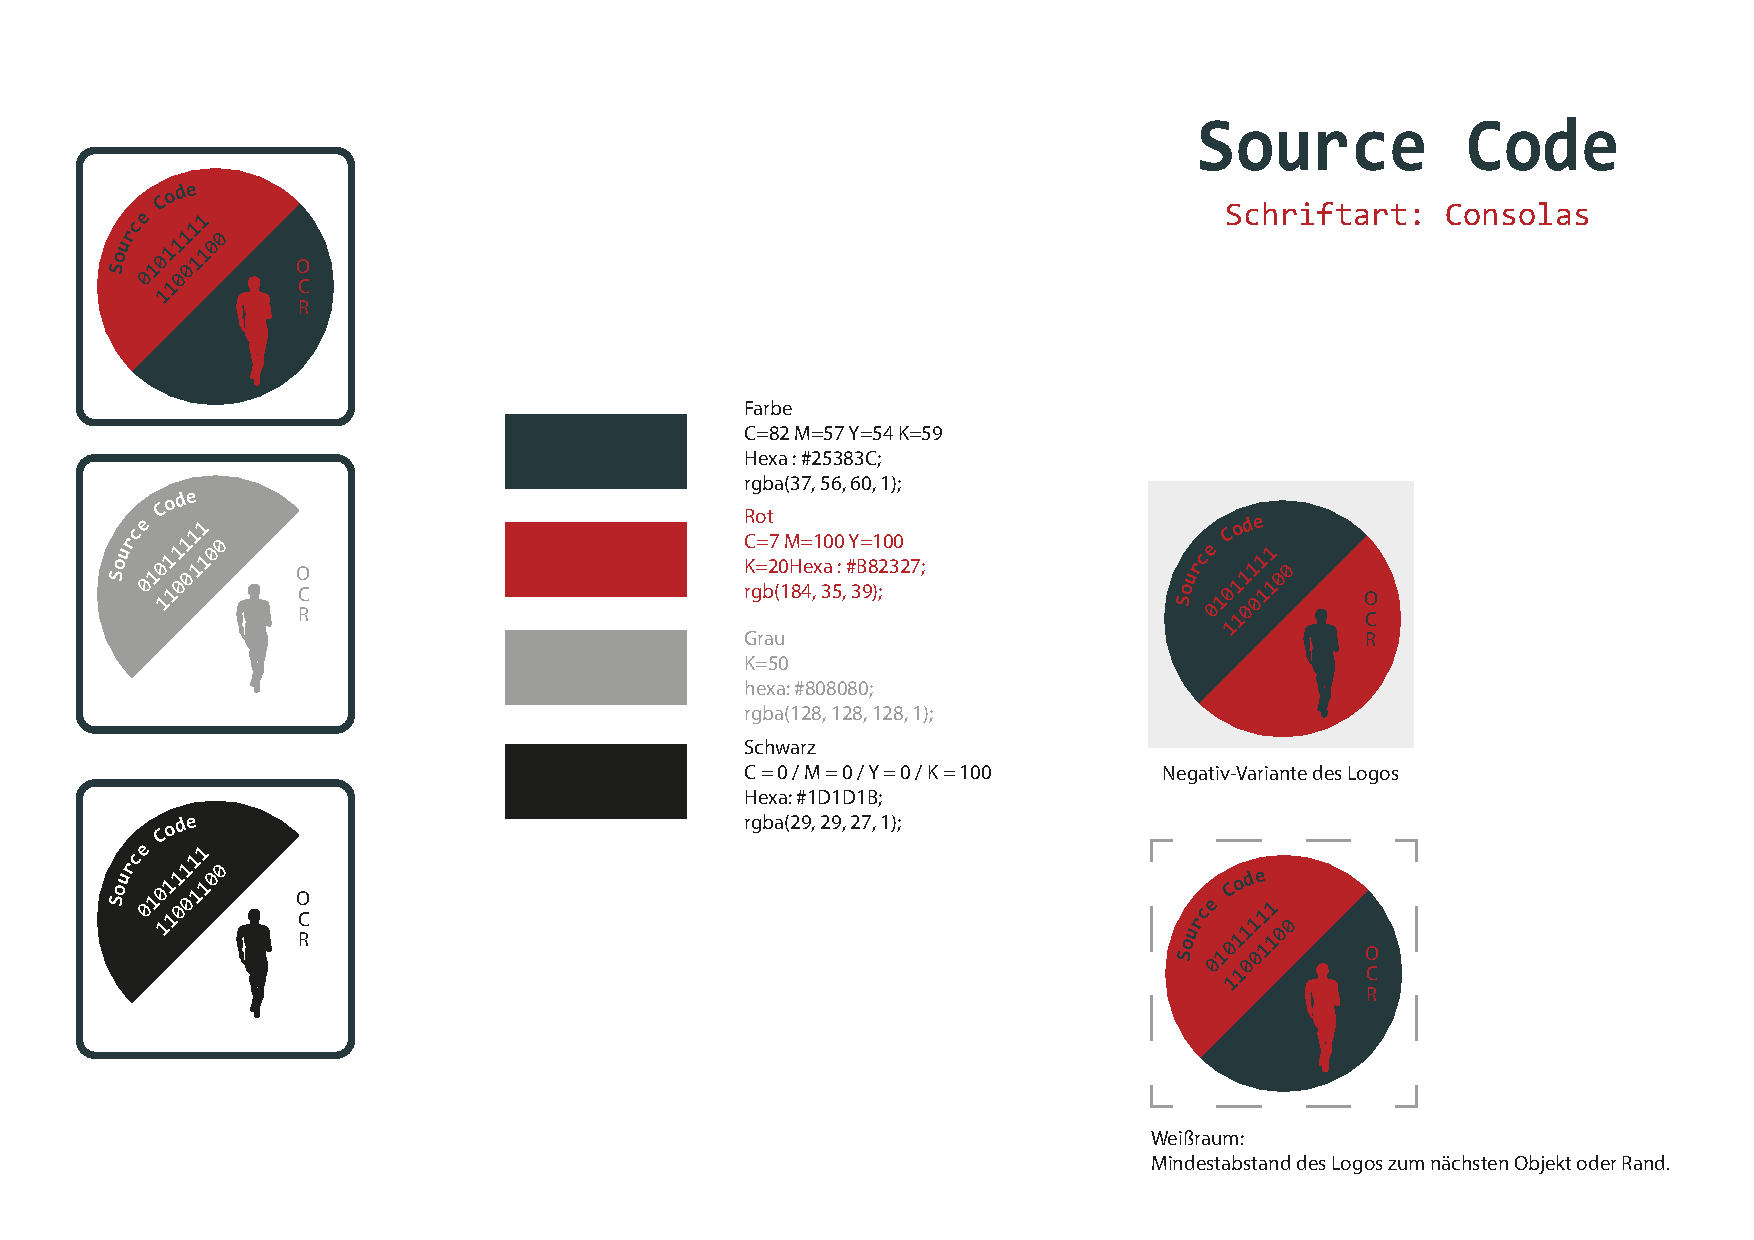
\includegraphics[width=.35\textwidth]{content/bsp/Logo-Details.pdf}
	%---------------------------------
	%\caption{Bild} \label{bild}
\end{figure}

Logo in Negativ, Grau u. Schwarz (siehe Abb. \ref{logo_negativ_grau_schwarz})
\begin{figure}[H]
	\centering
	\begin{minipage}[b]{0.40\textwidth}
		
\includegraphics[width=\textwidth]{content/bsp/Logo-negativ.pdf}
	\end{minipage}
	\hfill
	\begin{minipage}[b]{0.30\textwidth}
		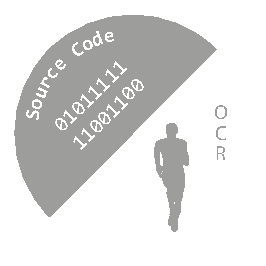
\includegraphics[width=\textwidth]{content/bsp/Logo-Grau.pdf}
	\end{minipage}
	\hfill
	\begin{minipage}[b]{0.20\textwidth}
		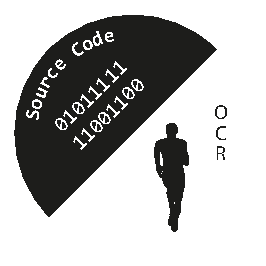
\includegraphics[width=\textwidth]{content/bsp/Logo-SW.pdf}
	\end{minipage}
	%---------------------------------
	\caption{Logo in Negativ, Grau u. Schwarz
		     \newline Quelle: https://www.ju1.eu/}
	\label{logo_negativ_grau_schwarz}
\end{figure}

Logo Details (siehe Abb. \ref{logo_details})
\begin{figure}[H]
	\centering
	\begin{minipage}[b]{0.49\textwidth}
		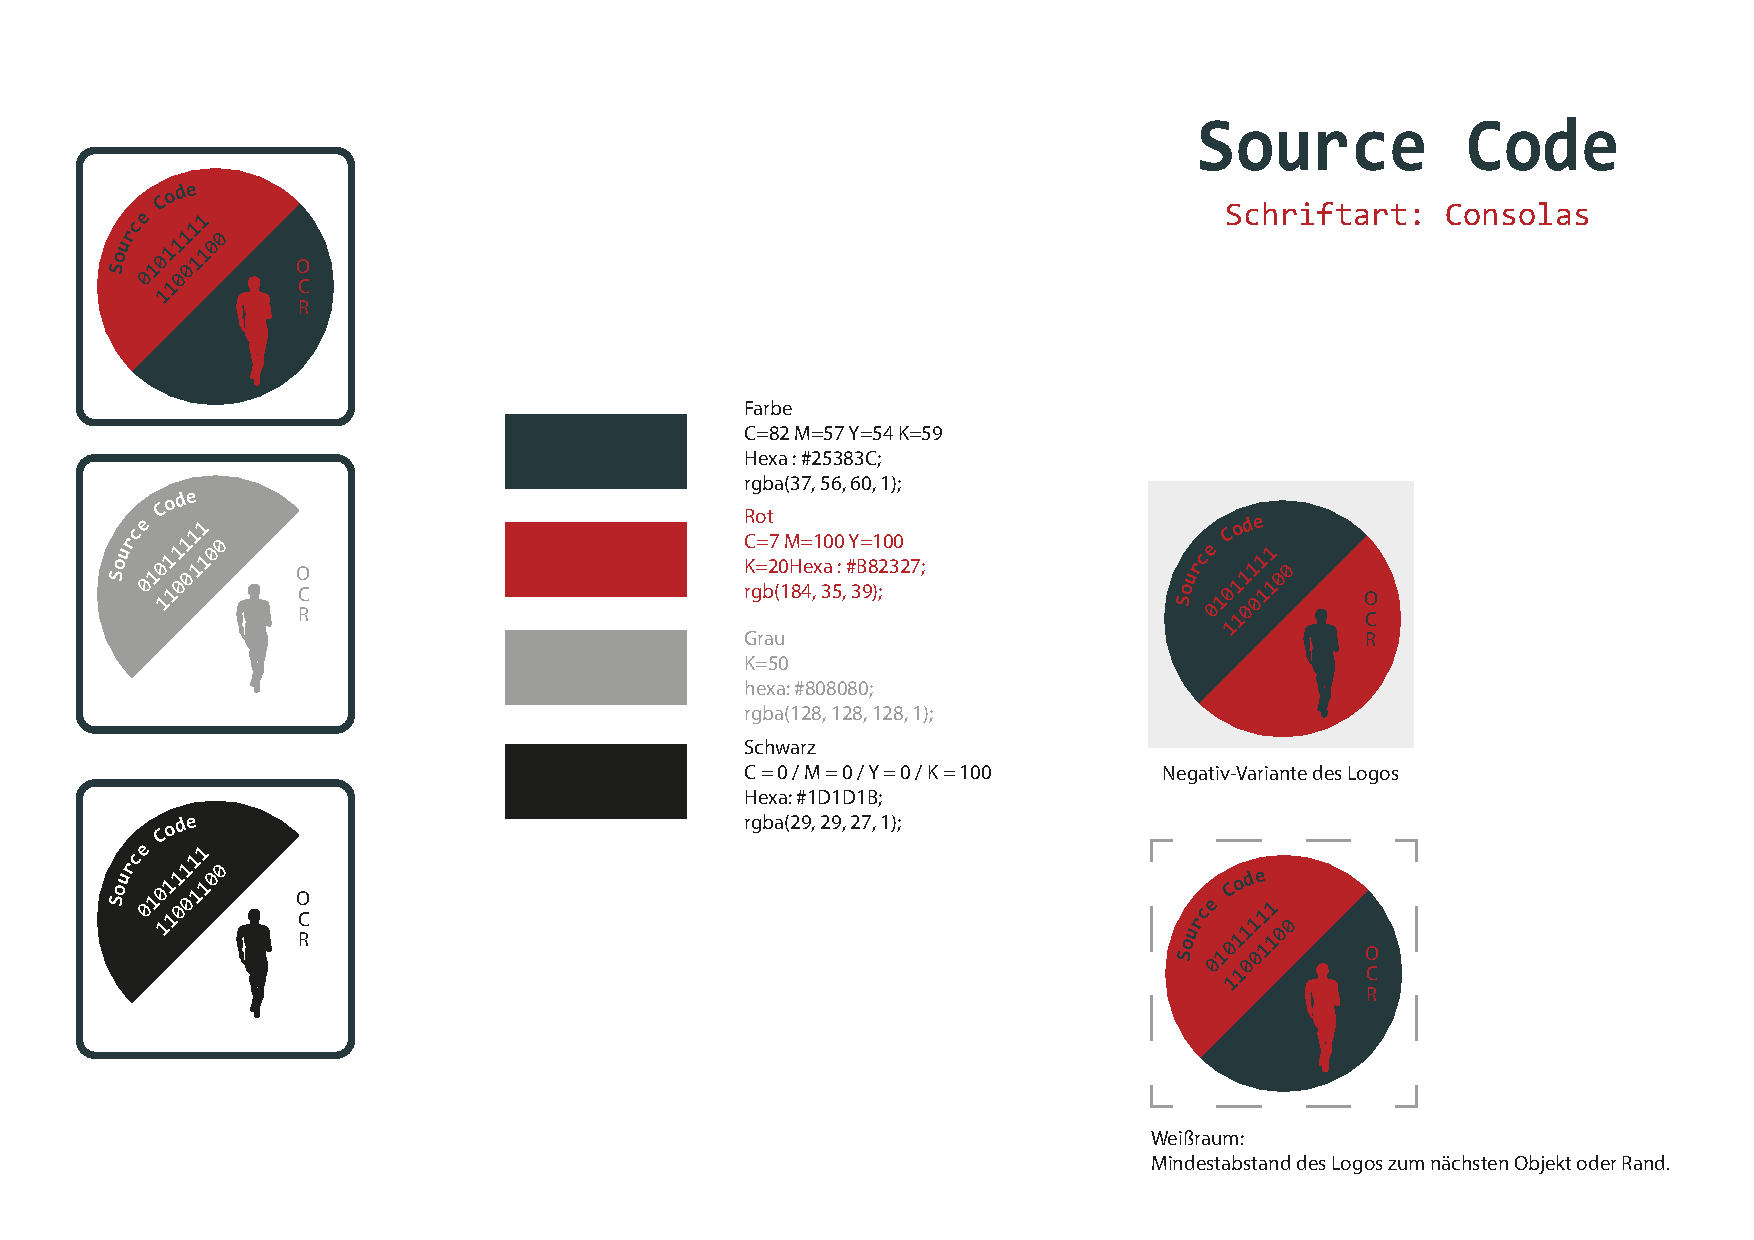
\includegraphics[width=\textwidth]{content/bsp/Logo-Details.pdf}
	\end{minipage}
	\hfill
	\begin{minipage}[b]{0.49\textwidth}
		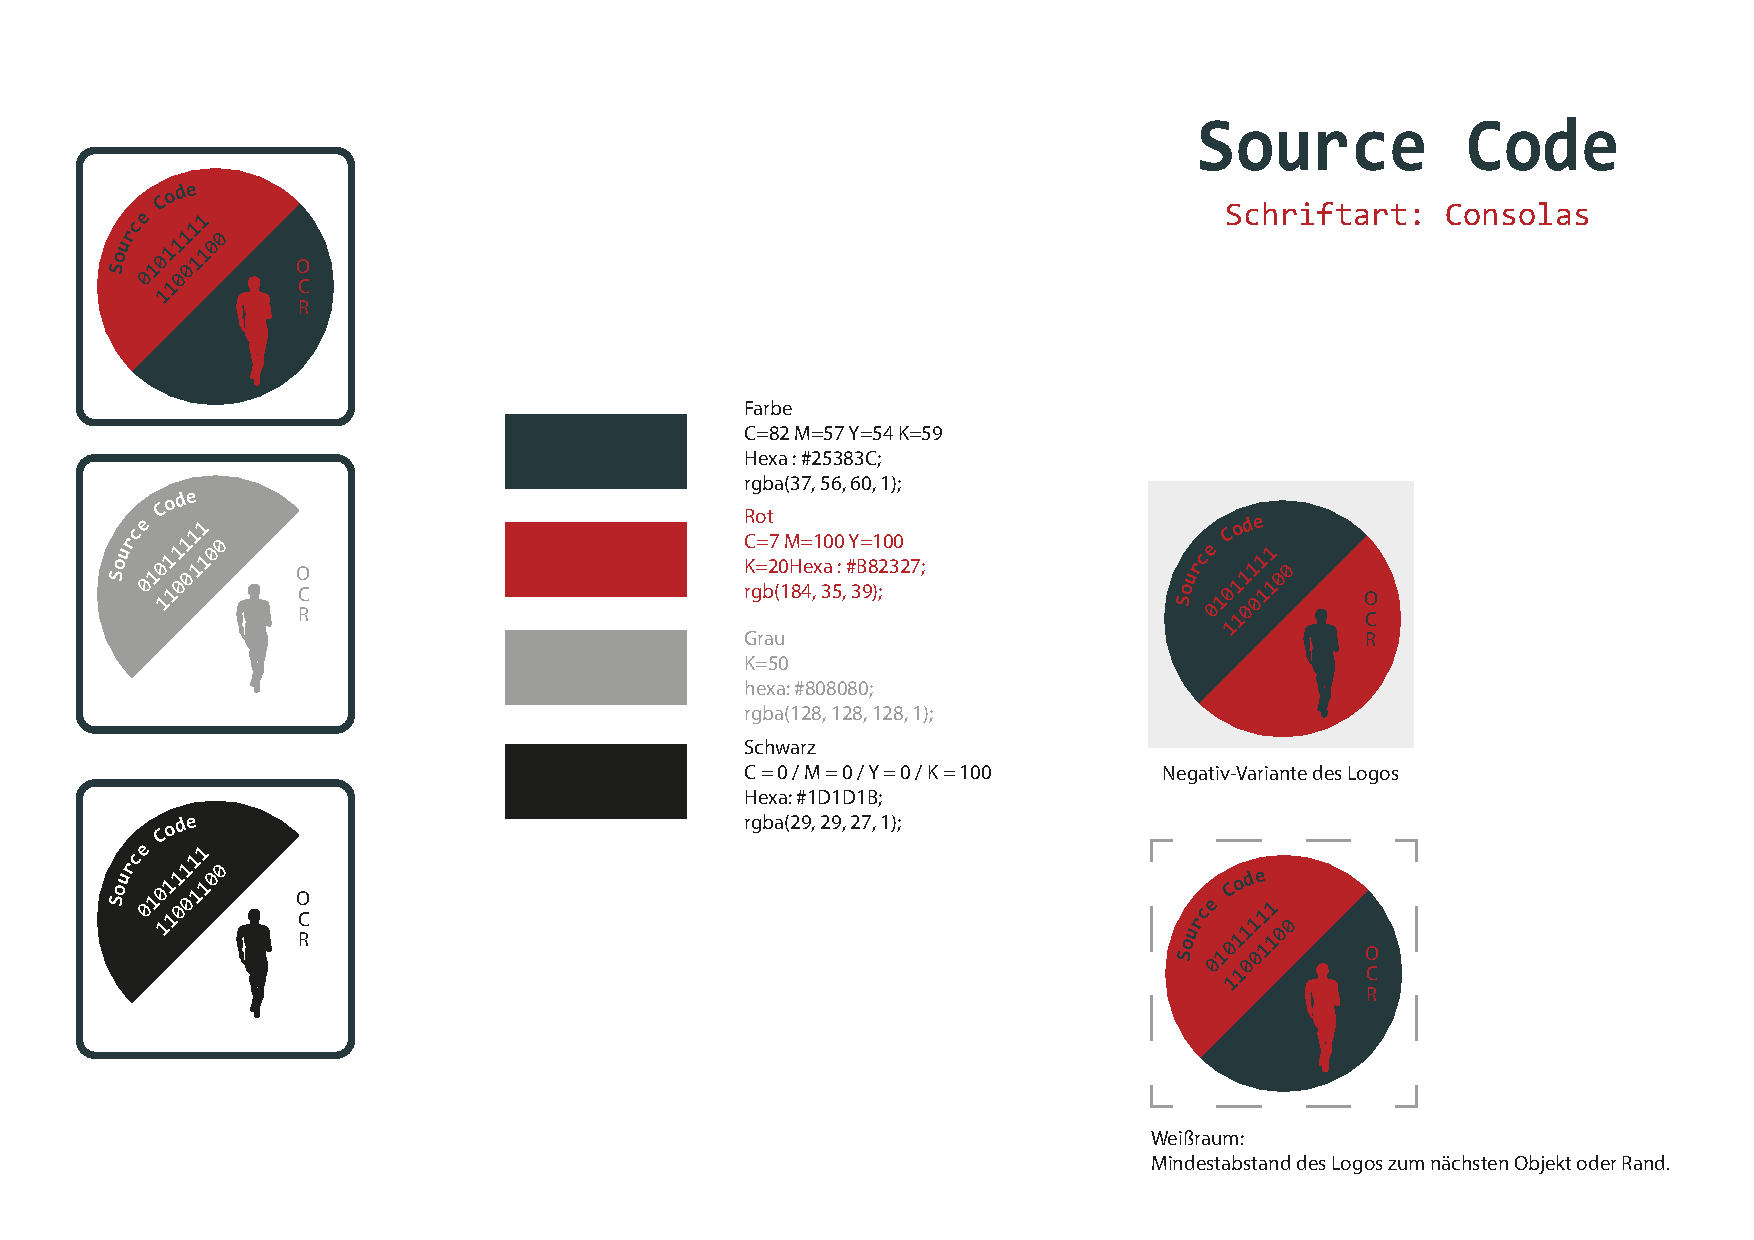
\includegraphics[width=\textwidth]{content/bsp/Logo-Details.pdf}
	\end{minipage}
	%---------------------------------
	\caption{Logo Details} \label{logo_details}
\end{figure}


\subsection{Tabelle}
\label{tabelle}

Tabelle (vgl. Tab. \ref{tabelle_}). 
\begin{table}[H]% hier: htbp
	\centering
	\arrayrulecolor{lightgray}
	\sffamily\footnotesize
	\begin{tabular}{ll}% Spalte: lcr 
		\toprule
		\textbf{Nr.} & \textbf{Vorgehen} \\
		\midrule
		1 & Aktuellen Forschungsstand recherchieren \\
		2 & Methoden entwickeln \\
		3 & Schlussfolgerung aufstellen \\
		\bottomrule
	\end{tabular}
	%---------------------------------
	\caption{Tabelle}\label{tabelle_}%
\end{table}

\bigskip
%\centering
\begin{tabular}[2]{|p{3cm}|p{9cm}|}
	\hline
	\textbf{Teil} & \textbf{Beschreibung} \\ \hline
	Batterie & Versorgt das System mit Strom. Hat einen ungeregelten Spannungsbereich von ca. 11,5 V - 16,75 V je nach Ladezustand \\ \hline
	Schalter & mechanische Trennung der elektrischen Energie zum Rest des Roboters \\ \hline
\end{tabular}
\bigskip

%\centering
\begin{tabular}[3] {| l | l | l |}
	\hline
	\textbf{Control Board Label} & \textbf{Wire Color} & \textbf{Signal} \\ \hline
	VCC & Red & Motor + \\ \hline
	GND & Black & GND \\ \hline
\end{tabular} 
\bigskip

%\centering
\begin{tabular}{|N|N|}
	\hline
	\textbf{Control Board pin} & \textbf{cable wire color} \\ \hline
	1. GND & Black \\ \hline
	2. 5V & Red \\ \hline
\end{tabular}
\bigskip

\begin{table}[H]
	\centering
	\arrayrulecolor{lightgray}
	\sffamily\footnotesize
	\begin{tabular}{|N|Q|Q|I|N|Q|Q|I|}
		\hline
		\thead{Artikel} & \thead{Ref} & \thead{Menge} & \thead{Bild} & 
		\thead{Artikel} & \thead{Ref} & \thead{Menge} & \thead{Bild} \\ \hline
		Battery & logo & 1 & \partimg{content/bsp/logo.pdf} & 
		Tamiya Connectors & logo & 1 & \partimg{content/bsp/logo.pdf} \\ \hline
		Battery Charger & logo & 1 & \partimg{content/bsp/logo.pdf} & & & & \\ \hline
	\end{tabular}
	%---------------------------------
	\caption{Komponenten} \label{komponenten}
\end{table}

\begin{table}[H]
	\centering
	\arrayrulecolor{lightgray}
	\sffamily\footnotesize
	\begin{tabular}[3] {| p{2cm} | p{5cm} | p{2cm} | }
		\hline
		\textbf{Pin} & \textbf{Description} & \textbf{Color} \\ \hline
		1 & +5V DC Power & \textcolor{red}{\textbf{Red}} \\ \hline
		2 & GND & \textcolor{black}{\textbf{Black}} \\ \hline
	\end{tabular}
	%---------------------------------
	\caption{Pinbelegung} \label{pinbelegung}
\end{table}

\begin{table}[H]
	\centering
	\arrayrulecolor{lightgray}
	\sffamily\footnotesize
	\begin{tabular}{|c|c|c|}
		\hline
		\thead{Item} & \thead{Ref} & \thead{Board Ref} \\ \hline
		4.7K 1/4 Watt Res & E7 & R1 \\ \hline
		10K 1/2 Watt Res & E10 & R2 \\ \hline
		100nF Cap & E11 & C1-17 \\ \hline
	\end{tabular}
	%---------------------------------
	\caption{Resistor/Capacitor reference}
\end{table}

\begin{centering}
	\begin{tabular}[2]{|c|c|}
		\hline
		\textbf{Variable} & \textbf{Physical description} \\ \hline
		$d_1$ & Horizontal distance \\ \hline
		$d_2$ & Vertical distance  \\ \hline
	\end{tabular}
	
	\begin{figure}[H]
		\centering
		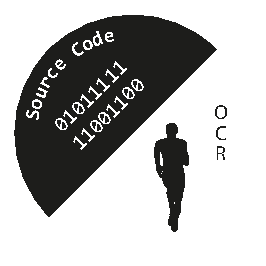
\includegraphics[width=.35\textwidth]{content/bsp/Logo-SW.pdf}
		%---------------------------------
		\caption{Physical distance} \label{r5}
	\end{figure}	
\end{centering}

\subsection{Formel}
\label{formel}

\begin{equation}
	d_1 = 7.254 mm \qquad d_2 = d_3 = 10.5 mm \qquad d_4 = 10.073 mm
\end{equation}

\begin{equation}
	1 \le 2 \ge 0 \neq 4, \quad 1 \ll 10^{20} \gg 10^{-5} \pm 
\end{equation}

\begin{equation}
	a \cdot b \quad
	a \times b \quad
	\frac x2 \quad
	a_1 \quad
	a^2 \quad
	\binom{a}{b} \quad
	\sqrt{x} \quad bzw. \quad \sqrt[n]{x} \quad	
\end{equation}

\begin{equation}
	\sum \limits_{i=1}^n i = \frac{n(n+1)}{2}
\end{equation}

\begin{equation}
	\prod \limits_{i=1}^{n+1}i = 1\cdot 2\cdot\dots\cdot n\cdot (n+1)
\end{equation}

\begin{equation}
	\lim\limits_{n \to \infty}\frac{1}{n}=0
\end{equation}

\begin{equation}
	\left(
		\begin{array}{ccc}
			a_{11} & \cdots & a_{1n} \\
			\vdots & \ddots & \vdots \\
			a_{m1} & \cdots & a_{mn}
		\end{array}
	\right)	
\end{equation}

\subsection{Textauszeichnung}
\label{textauszeichnung}

\textbf{fetter Text}

\textbf{**Hinweis** Diese haben NICHT die gleiche Farbe und Pinbelegung wie die Antriebsmotoren!}


\subsection{Farben}
\label{farben}

\begin{itemize}
	%\textcolor{}{}
	%\item[] \colorbox{}{}
	\item[] \colorbox{Apricot}{Apricot} \colorbox{Aquamarine}{Aquamarine}
            \textcolor{Apricot}{Apricot}
	\item[] Apricot		Cyan		Mahogany		ProcessBlue		SpringGreen
	\item[] Aquamarine		Dandelion		Maroon		Purple		Tan
	\item[] BitterSweet		DarkOrchid		Melon		RawSienna		TealBlue
	\item[] Black		Emerald		MidnightBlue		Red		Thistle
	\item[] Blue		ForestGreen		Mulberry		RedOrange		Turquoise
	\item[] BlueGreen		Fuchsia		NavyBlue		RedViolet		Violet
	\item[] BlueViolet		Goldenrod		OliveGreen		Rhodamine		VioletRed
	\item[] Brickred		Gray		Orange		RoyalBlue		White
	\item[] Brown		Green		OrangeRed		RoyalPurple		WildStrawberry
	\item[] BurntOrange		GreenYellow		Orchid		RubineRed		Yellow
	\item[] CadetBlue		JungleGreen		Peach		Salmon		YellowGreen
	\item[] CarnationPink	Lavender	Periwinkle	SeaGreen YellowOrange
	\item[] Cerulean		LimeGreen		PineGreen		Sepia
	\item[] CornflowerBlue	Magenta	 Plum	SkyBlue
\end{itemize} 


\subsection{Zusammenfassung}
\label{zusammenfassung}

\mybox{
	Es gibt ein paar wichtige Dinge, die beachtet werden sollten, wie bei jedem Projekt, bei dem mit Batterie oder elektrischem Strom gearbeitet wird:
	\newline
	\noindent \textbf{DIE BATTERIE}. 
}
	% ---------------------------------
% Latex Kapitel 
% ju - Letztes Update: 24-Dez-2019
% ---------------------------------
%
%\chapter{neu}
% letztes Update: 24-Dez-19
\section{Neu}\label{neu}

\clearpage
%\chapter{Quellcode-files}
%\input{Quellcode-files}
%\clearpage
%\chapter{Projekt-files}
%\input{Projekt-files}
%\clearpage


	% Beispiel
	%% FILE: kap01.tex  Version 1.0
% AUTHOR:
% letztes Update: 18-Mai-2019

%\section{\LaTeX}

\section{Zitieren}\label{zitieren}

Literaturlistenverwaltungsprogramm: JabRef 

% \cite{Schlüsselwort}
% \nocite{Schlüsselwort}

\nocite{*} Auch unzitierte Literatur wird gedruckt \verb|\nocite{*}|

Zitat: vgl. \cite{monk_action_buch:2016} u. \cite{kofler_linux:2017} 

\verb|vgl. \cite{monk_action_buch:2016} u. \cite{kofler_linux:2017}| 


\section{Links}\label{sec:links}

Verweis auf eine URL im Internet: 

\url{https://www.google.de/}
\verb|\url{https://www.google.de/}|

\href{https://www.google.de/}{google}
\verb|\href{https://www.google.de/}{google}|


\href{mailto:xx@yy.eu}{(E-Mail)} 
\verb|\href{mailto:xx@yy.eu}{(E-Mail)}|


\href{file:content/bsp/logo.pdf}{\fcolorbox{gruen-dunkel}{gruen-hell}{logo.pdf}}
\verb|\href{file:content/bsp/logo.pdf}|

\href{file:content/bsp/hallo.c}{\fcolorbox{rot-dunkel}{rot-hell}{hallo.c}}
\verb|\href{file:content/bsp/hallo.c}|

%\href{run:content/bsp/video.mp4}{\fcolorbox{blau-dunkel}{blau-hell}{video.mp4}}
%\verb|\href{run:content/bsp/video.mp4}|

\section{Fußnote}

Text\footnote{Fußnote} Text
\verb|\footnote{Fußnote}|

\section{Referenzieren}\label{referenzieren}

Verweis auf eine andere Stelle im selben Dokument:

Labeln von Section: Kapitel~(\ref{labelname}) oder (vgl.~\ref{zitieren}) 

Labeln von Titel: vgl.~(\nameref{labelname}) 

Labeln von Bildern: (vgl.~\ref{fig:latexproduktion}) 

Labeln von Tabellen: (vgl.~\ref{tab:tabelle}) 

Labeln von Quellcode: (vgl.~\ref{code:lstlisting}) 

Labeln von Gleichungen: Formeln~\ref{eq:ekin} und \ref{eq:impuls}

\LaTeX -Syntax (vgl.~\ref{code:referenzieren}). 
\begin{lstlisting}[caption={Referenzieren},label={code:referenzieren},language=TeX% C, TeX, Bash, Python
]-----Code einfügen---------------------------%
	Labeln von Section-Nr: Kapitel~(\ref{labelname}) oder (vgl.~\ref{zitieren}) 
	Labeln von Titel: vgl.~(\nameref{labelname}) 
	Labeln von Bildern: (vgl.~\ref{fig:latexproduktion}) 
	Labeln von Tabellen: (vgl.~\ref{tab:tabelle}) 
	Labeln von Quellcode: (vgl.~\ref{code:lstlisting}) 
	Labeln von Gleichungen: Formeln~\ref{eq:ekin} und \ref{eq:impuls}
\end{lstlisting}

\section{Randnotiz}

Randnotiz: \marginpar[links]{rechts} 
\verb|\marginpar[links]{rechts}| 

\section{Index}
	
Indexeintrag: \index{Eintragsname!Untereintrag} 
\verb|\index{Eintragsname!Untereintrag}|

\section{Eigene Befehle - Abstand}

\wichtig{xxx} \wort{yyy} \fremdwort{zzz} 
\verb|\wichtig{xxx} \wort{yyy} \fremdwort{zzz}|

horizontaler $\cdots$ \abstand{$\cdots$ Abstand}

horizontaler Abstand $\cdots$ \hspace{2em} $\cdots$ Abstand

vertikaler Abstand $\cdots$\\
\vspace{3em}\\
$\cdots$ Abstand

\verb|\hspace{2em} vspace{3em}|

% Abstand
Abstand
\vfill
Abstand \hfill \today\\
Abstand \hfil \today

\section{PDF/A-1b erzeugen}\label{labelname}

\begin{itemize}
	\item Öffne die PDF-Datei mit Adobe Acrobat Pro.
	\item In Acrobat Pro auf Werkzeuge / PDF-Standards / Preflight klicken
	\item Suche im Preflight-Fenster nach <<Nach PDF/A-1b konvertieren>>,
	welches sich in der Gruppe <<PDF/A-Standard>> befindet.
	\item Starte die Konvertierung durch Doppelklick auf das Profil.
	\item Es erscheint ein neues Fenster, gebe dort einen neuen Dateinamen ein
	\item Wenn keine Fehler angezeigt werden, ist die neue Datei ein PDF/A-1b-konformes Dokument.	
\end{itemize}

\clearpage
\section{Blindtext}
\blindtext

\blindtext

\clearpage
\section{Tabelle}

(vgl.~\ref{tab:tabelle}). 
\begin{table}[ht]% hier: htbp
	\centering
	\begin{tabular}{ll}% Spalte: lcr 
		\toprule
		\textbf{Nr.} & \textbf{Vorgehen} \\
		\midrule
		1 & Aktuellen Forschungsstand recherchieren \\
		2 & Methoden entwickeln \\
		3 & Schlussfolgerung aufstellen \\
		\bottomrule
	\end{tabular}
	%------------------------------------
	\caption{Tabelle}\label{tab:tabelle}%
\end{table}

\LaTeX -Syntax (vgl.~\ref{code:tabelle}). 
\begin{lstlisting}[caption={\LaTeX: Tabelle},label={code:tabelle},language=TeX% C, TeX, Bash, Python
]-----Code einfügen---------------------------%
	\begin{table}[ht]% hier: htbp
		\centering
		\begin{tabular}{ll}% Spalte: lcr 
			\toprule
			\textbf{Nr.} & \textbf{Vorgehen} \\
			\midrule
			1 & Aktuellen Forschungsstand recherchieren \\
			2 & Methoden entwickeln \\
			3 & Schlussfolgerung aufstellen \\
			\bottomrule
		\end{tabular}
		%------------------------------------
		\caption{\LaTeX: Tabelle}\label{tab:tabelle}%
	\end{table}
\end{lstlisting}

\clearpage
\section{Abbildung}\label{abbildung}

(vgl.~\ref{fig:latexproduktion})
\begin{figure}[hb]% hier: htbp
	\centering
	
\includegraphics[width=0.2\textwidth]{content/bsp/logo.pdf}
	%------------------------------------
	\caption{Latexproduktion}\label{fig:latexproduktion}% 
\end{figure}

\LaTeX -Syntax (vgl.~\ref{code:abbildung}). 
\begin{lstlisting}[caption={\LaTeX: Abbildung},label={code:abbildung},language=TeX% C, TeX, Bash, Python
]-----Code einfügen---------------------------%
	\begin{figure}[hb]% hier: htbp
		\centering
		
\includegraphics[width=0.2\textwidth]{content/bsp/logo.pdf}
		%------------------------------------
		\caption{Latexproduktion}\label{fig:latexproduktion}% 
	\end{figure}
\end{lstlisting}

\clearpage
Zwei Bilder nebeneinander (vgl.~\ref{fig:subfigure}). 
\begin{figure}
	\centering
	\begin{subfigure}[b]{0.2\textwidth}
		\centering
		
\includegraphics[width=\textwidth]{content/bsp/logo.pdf}
		\subcaption{Bild 1}	
	\end{subfigure}
	\begin{subfigure}[b]{0.2\textwidth}
		\centering
		
\includegraphics[width=\textwidth]{content/bsp/logo.pdf}
		\subcaption{Bild 2}
	\end{subfigure}
	\caption{Zwei Bilder nebeneinander}\label{fig:subfigure}
\end{figure}

\LaTeX -Syntax (vgl.~\ref{code:subfigure}). 
\begin{lstlisting}[caption={subfigure},label={code:subfigure},language=TeX% C, TeX, Bash, Python
]-----Code einfügen---------------------------%
	\begin{figure}
		\centering
		\begin{subfigure}[b]{0.2\textwidth}
			\centering
			
\includegraphics[width=\textwidth]{content/bsp/logo.pdf}
			\subcaption{Bild 1}	
		\end{subfigure}
		\begin{subfigure}[b]{0.2\textwidth}
			\centering
			
\includegraphics[width=\textwidth]{content/bsp/logo.pdf}
			\subcaption{Bild 2}
		\end{subfigure}
		\caption{Zwei Bilder nebeneinander}
	\end{figure}
\end{lstlisting}

\clearpage
\section{Farben - Hinweis}

% Text läuft über Seitenrand, wenn zu lang
\fbox{kurzer farbiger Text}\\
\colorbox{rot2}{kurzer farbiger Text}\\
\fcolorbox{gruen-dunkel}{gruen-hell}{kurzer farbiger Text}\\

\textbf{\textcolor{rot2}{fetter Text in Farbe}}

\LaTeX -Syntax (vgl.~\ref{code:farben}). 
\begin{lstlisting}[caption={Farben},label={code:farben},language=TeX% C, TeX, Bash, Python
]-----Code einfügen---------------------------%
	% Text läuft über Seitenrand, wenn zu lang
	\fbox{kurzer farbiger Text}\\
	\colorbox{rot2}{kurzer farbiger Text}\\
	\fcolorbox{gruen-dunkel}{gruen-hell}{kurzer farbiger Text}\\	
	\textbf{\textcolor{rot2}{fetter Text in Farbe}}
\end{lstlisting}

\begin{quote}
	\textbf{Hinweis:}\\%
	Auch gibt es niemanden, der den Schmerz an sich liebt, sucht oder wünscht, nur, weil er Schmerz ist, es sei denn, es kommt zu zufälligen Umständen, in denen Mühen und Schmerz ihm große Freude bereiten können. Um ein triviales Beispiel zu nehmen, wer von uns unterzieht sich je anstrengender körperlicher
\end{quote}

\LaTeX -Syntax (vgl.~\ref{code:Hinweis-quote}). 

\begin{lstlisting}[caption={Hinweis in quote},label={code:Hinweis-quote},language=TeX% C, TeX, Bash, Python
]-----Code einfügen---------------------------%
	\begin{quote}
		\textbf{Hinweis:}\\%
		Text
	\end{quote}
\end{lstlisting}

\clearpage
\begin{figure}[hb]
	\centering
	\begin{minipage}[b]{0.88\textwidth} 
		\color{blau5}\rule{\textwidth}{2pt}\\%
		\textbf{Hinweis:}\\
		Auch gibt es niemanden, der den Schmerz an sich liebt, sucht oder wünscht, nur, weil er Schmerz ist, es sei denn, es kommt zu zufälligen Umständen, in denen Mühen und Schmerz ihm große Freude bereiten können. Um ein triviales Beispiel zu nehmen, wer von uns unterzieht sich je anstrengender körperlicher
		\\ \rule{\textwidth}{2pt}%
		% \caption{}\label{}
	\end{minipage}
	% \caption{}\label{}
\end{figure}

\LaTeX -Syntax (vgl.~\ref{code:Hinweis-minipage}). 

\begin{lstlisting}[caption={Hinweis in minipage},label={code:Hinweis-minipage},language=TeX% C, TeX, Bash, Python
]-----Code einfügen---------------------------%
	\begin{figure}[hb]
		\centering
		\begin{minipage}[b]{0.88\textwidth} 
			\color{blau5}\rule{\textwidth}{2pt}\\%
			\textbf{Hinweis:}\\
			Text
			\\ \rule{\textwidth}{2pt}%
			% \caption{}\label{}
		\end{minipage}
		% \caption{}\label{}
	\end{figure}
\end{lstlisting}

\begin{figure}[hb]
	\centering
	\fcolorbox{rot-dunkel}{rot4}{% Rahmen
		\begin{minipage}[b]{0.88\textwidth} 
			\color{white}
			\textbf{Hinweis:}\\%
			Auch gibt es niemanden, der den Schmerz an sich liebt, sucht oder wünscht, nur, weil er Schmerz ist, es sei denn, es kommt zu zufälligen Umständen, in denen Mühen und Schmerz ihm große Freude bereiten können. Um ein triviales Beispiel zu nehmen, wer von uns unterzieht sich je anstrengender körperlicher
			% \caption{}\label{}
		\end{minipage}
	}
	% \caption{}\label{}
\end{figure}

\LaTeX -Syntax (vgl.~\ref{code:Hinweis-fcolorbox}). 

\begin{lstlisting}[caption={Hinweis in fcolorbox},label={code:Hinweis-fcolorbox},language=TeX% C, TeX, Bash, Python
]-----Code einfügen---------------------------%
	\begin{figure}[hb]
		\centering
		\fcolorbox{rot-dunkel}{rot4}{% Rahmen
			\begin{minipage}[b]{0.88\textwidth} 
				\color{white}
				\textbf{Hinweis:}\\%
				Text
				% \caption{}\label{}
			\end{minipage}
		}
		% \caption{}\label{}
	\end{figure}
\end{lstlisting}

\clearpage
\section{Quellcode}

\LaTeX -Syntax (vgl.~\ref{code:lstlisting}). 

\begin{lstlisting}[caption={lstlisting},label={code:lstlisting},language=TeX% C, TeX, Bash, Python
]-----Code einfügen---------------------------%
	% Code
\end{lstlisting}


\lstinputlisting[caption={C-Programmierung},language=C]{content/bsp/hallo.c}

\LaTeX -Syntax (vgl.~\ref{code:lstinputlisting}). 

\begin{lstlisting}[caption={lstinputlisting},label={code:lstinputlisting},language=TeX% C, TeX, Bash, Python
]-----Code einfügen---------------------------%
	% Code
	\lstinputlisting[language=C]{content/bsp/hallo.c}% file
\end{lstlisting}

\clearpage
\begin{figure}[hb]
	\centering
	\fcolorbox{gruen-dunkel}{gruen-hell}{% Rahmen
		\begin{minipage}[b]{0.5\textwidth} 
			\lstinputlisting[caption={Hallo Welt},language=C]{content/bsp/hallo.c}
			% \caption{}\label{}
		\end{minipage}
	}
	% \caption{} \label{}
\end{figure}

\LaTeX -Syntax (vgl.~\ref{code:code-rahmen}). 

\begin{lstlisting}[caption={Code im Rahmen},label={code:code-rahmen},language=TeX% C, TeX, Bash, Python
]-----Code einfügen---------------------------%
	\begin{figure}[hb]
		\centering
		\fcolorbox{gruen-dunkel}{gruen-hell}{% Rahmen
		\begin{minipage}[b]{0.5\textwidth} 
			\textbf{Code:}\\%
			\lstinputlisting[language=C]{content/bsp/hallo.c}
			% \caption{}\label{}
		\end{minipage}
		}
		% \caption{} \label{}
	\end{figure}
\end{lstlisting}

\clearpage
\section{Gliederung}

\LaTeX -Syntax (vgl.~\ref{code:gliederung}).

\begin{lstlisting}[language=TeX,% C, TeX, Bash, Python
	caption={Gliederung},label={code:gliederung}%
]-----Code einfügen---------------------------%
	% Kapitel:
	\chapter \section \subsection \subsubsection \paragraph 
\end{lstlisting}

\clearpage
\section{Minipage}

\textbf{zwei Texte nebeneinander}\\

\begin{figure}[hb]
	\centering
	\fbox{% Rahmen
		\begin{minipage}[t]{0.4\textwidth} 
			Auch gibt es niemanden, der den Schmerz an sich liebt, sucht oder wünscht, nur, weil er Schmerz ist, es sei denn, es kommt zu zufälligen Umständen, in denen Mühen und Schmerz ihm große Freude bereiten können. Um ein triviales Beispiel zu nehmen, wer von uns unterzieht sich je anstrengender körperlicher
			% \caption{}\label{}
		\end{minipage}
	}
	\hfil
	\fcolorbox{gruen-dunkel}{gruen-hell}{% Rahmen
		\begin{minipage}[t]{0.4\textwidth}
			Auch gibt es niemanden, der den Schmerz an sich liebt, sucht oder wünscht, nur, weil er Schmerz ist, es sei denn, es kommt zu zufälligen Umständen, in denen Mühen und Schmerz ihm große Freude bereiten können. Um ein triviales Beispiel zu nehmen, wer von uns unterzieht sich je anstrengender körperlicher
			% \caption{}\label{}
		\end{minipage}
	}
	% \caption{}\label{}
\end{figure}

\LaTeX -Syntax (vgl.~\ref{code:zwei-texte-nebeneinander}). 
\begin{lstlisting}[caption={zwei Texte nebeneinander },label={code:zwei-texte-nebeneinander},language=TeX% C, TeX, Bash, Python
]-----Code einfügen---------------------------%
	\begin{figure}[hb]
		\centering
		\fbox{% Rahmen
		\begin{minipage}[t]{0.4\textwidth} 
			Text
			% \caption{}\label{}
		\end{minipage}
		}
		\hfil
		\fcolorbox{gruen-dunkel}{gruen-hell}{% Rahmen
		\begin{minipage}[t]{0.4\textwidth}
			Text
			% \caption{}\label{}
		\end{minipage}
		}
		% \caption{}\label{}
	\end{figure}
\end{lstlisting}

\clearpage
\textbf{Text und Abb. nebeneinander}\\

\begin{figure}[hb]
	\centering
	\fbox{% Rahmen
		\begin{minipage}[b]{0.5\textwidth} 
			Auch gibt es niemanden, der den Schmerz an sich liebt, sucht oder wünscht, nur, weil er Schmerz ist, es sei denn, es kommt zu zufälligen Umständen, in denen Mühen und Schmerz ihm große Freude bereiten können. 
			\\\\
			Auch gibt es niemanden, der den Schmerz an sich liebt, sucht oder wünscht, nur, weil er Schmerz ist, es sei denn, es kommt zu zufälligen Umständen, in denen Mühen und Schmerz ihm große Freude bereiten können.
			% \caption{}\label{}
		\end{minipage}
	}
	\hfil
	%\fbox
	% \caption{}\label{}
\end{figure}

\LaTeX -Syntax (vgl.~\ref{code:Text-Abb})

\begin{lstlisting}[language=TeX,% C, TeX, Bash, Python
caption={Text und Abb. nebeneinander},label={code:Text-Abb}%
]-----Code einfügen---------------------------%
	\begin{figure}[hb]
		\centering
		\fbox{% Rahmen
		\begin{minipage}[b]{0.5\textwidth} 
			Text
			% \caption{}\label{}
		\end{minipage}
		}
		\hfil
		%\fbox
		% \caption{}\label{}
	\end{figure}
\end{lstlisting}

\clearpage
\textbf{Liste und Abbildung nebeneinander}\\

\begin{figure}[hb]
	\centering
	\fbox{% Rahmen
		\begin{minipage}[b]{0.5\textwidth} 
			\begin{itemize}
				\item Listenpunkt a
				\begin{itemize}
					\item Listenpunkt c
					\begin{itemize}
						\item Listenpunkt d
					\end{itemize}
				\end{itemize}
				\item Listenpunkt b
			\end{itemize}
			% \caption{}
			% \label{}
		\end{minipage}
	}
	\hfil
	%\fbox
	% \caption{}
	% \label{}
\end{figure}

\LaTeX -Syntax (vgl.~\ref{code:Liste-Abb})

\begin{lstlisting}[language=TeX,% C, TeX, Bash, Python
caption={Liste und Abb. nebeneinander},label={code:Liste-Abb}%
]-----Code einfügen---------------------------%
	\begin{figure}[hb]
		\centering
		\fbox{% Rahmen
		\begin{minipage}[b]{0.5\textwidth} 
			\begin{itemize}
				\item Listenpunkt a
				\begin{itemize}
					\item Listenpunkt c
					\begin{itemize}
						\item Listenpunkt d
					\end{itemize}
				\end{itemize}
				\item Listenpunkt b
			\end{itemize}
			% \caption{}\label{}
		\end{minipage}
		}
		\hfil
		%\fbox
		% \caption{}\label{}
	\end{figure}
\end{lstlisting}

\clearpage
\textbf{Text und Code nebeneinander}\\

\begin{figure}[hb]
	\centering
	%\fbox{
	\begin{minipage}[b]{0.45\textwidth}
		Auch gibt es niemanden, der den Schmerz an sich liebt, sucht oder wünscht, nur, weil er Schmerz ist, es sei denn, es kommt zu zufälligen Umständen, in denen Mühen und Schmerz ihm große Freude bereiten können. Um ein triviales Beispiel zu nehmen, wer von uns unterzieht sich je anstrengender körperlicher
		% \caption{}
		% \label{}
	\end{minipage}
	%}
	\hfil
	\fcolorbox{gruen-dunkel}{gruen-hell}{% Rahmen
		\begin{minipage}[b]{0.45\textwidth} 
			\textbf{Code:}\\%
			\lstinputlisting[caption={Ein kleines Programm in C},language=C]
			{content/bsp/hallo.c}
			% \caption{}
			% \label{}
		\end{minipage}
	}
	% \caption{}
	% \label{}
\end{figure}

\LaTeX -Syntax (vgl.~\ref{code:Text-Code})

\begin{lstlisting}[language=TeX,% C, TeX, Bash, Python
caption={Text und Code nebeneinander},label={code:Text-Code}%
]-----Code einfügen---------------------------%
	\begin{figure}[hb]
		\centering
		%\fbox{
		\begin{minipage}[b]{0.45\textwidth}
			Text
			% \caption{}\label{}
		\end{minipage}
		%}
		\hfil
		\fcolorbox{gruen-dunkel}{gruen-hell}{% Rahmen
		\begin{minipage}[b]{0.45\textwidth} 
			\textbf{Code:}\\%
			\lstinputlisting[caption={Ein kleines Programm in C},language=C]
			{content/bsp/hallo.c}
			% \caption{}\label{}
		\end{minipage}
		}
		% \caption{}\label{}
	\end{figure}
\end{lstlisting}


\clearpage
\section{Liste}

\begin{itemize}
	\item Listenpunkt a
	\begin{itemize}
		\item Listenpunkt c
		\begin{itemize}
			\item Listenpunkt d
		\end{itemize}
	\end{itemize}
	\item Listenpunkt b
\end{itemize}


\LaTeX -Syntax (vgl.~\ref{code:Liste})

\begin{lstlisting}[language=TeX,% C, TeX, Bash, Python
caption={Liste},label={code:Liste}%
]-----Code einfügen---------------------------%
	\begin{itemize}
		\item Listenpunkt a
		\begin{itemize}
			\item Listenpunkt c
			\begin{itemize}
				\item Listenpunkt d
			\end{itemize}
		\end{itemize}
		\item Listenpunkt b
	\end{itemize}	
\end{lstlisting}

\clearpage
\section{Textcommands}

50~Euro\\
Google-Account\\
Seite 42--45\\
Gedankenstrich --- falls\\
Mathe Minus $-1$\\
Hier ist ein Satz\ldots und so geht es weiter.\\
Hier ist ein Satz\ldots ~und so geht es weiter.\\
\textbf{fetter Text}
\textit{Text in Kursiv}
\textbf{\textit{fetter Text in Kursiv}}\\
\emph{Text betonen}


\LaTeX -Syntax (vgl.~\ref{code:textcommands})

\begin{lstlisting}[language=TeX,% C, TeX, Bash, Python
caption={Textcommands},label={code:textcommands}%
]-----Code einfügen---------------------------%
	50~Euro\\
	Google-Account\\
	Seite 42--45\\
	Gedankenstrich --- falls\\
	Mathe Minus $-1$\\
	Hier ist ein Satz\ldots und so geht es weiter.\\
	Hier ist ein Satz\ldots ~und so geht es weiter.\\
	\textbf{fetter Text}
	\textit{Text in Kursiv}
	\textbf{\textit{fetter Text in Kursiv}}\\
	\emph{Text betonen}
\end{lstlisting}

\clearpage
\section{Schriftgrößen}

% klein
\tiny Schriftgröße klein
\scriptsize Schriftgröße 
\footnotesize Schriftgröße
\small Schriftgröße\\
% normal
\normalsize Schriftgröße normal\\
% groß
\large Schriftgröße
\Large Schriftgröße
\LARGE Schriftgröße
\huge Schriftgröße
\Huge Schriftgröße groß\\

% normal
\normalsize Schriftgröße normal\\

\LaTeX -Syntax (vgl.~\ref{code:schriftgroessen})

\begin{lstlisting}[language=TeX,% C, TeX, Bash, Python
caption={Schriftgrößen},label={code:schriftgroessen}%
]-----Code einfügen---------------------------%
	% klein
	\tiny Schriftgröße klein
	\scriptsize Schriftgröße 
	\footnotesize Schriftgröße
	\small Schriftgröße\\
	% normal
	\normalsize Schriftgröße normal\\
	% groß
	\large Schriftgröße
	\Large Schriftgröße
	\LARGE Schriftgröße
	\huge Schriftgröße
	\Huge Schriftgröße groß\\
	
	% normal
	\normalsize Schriftgröße normal\\
\end{lstlisting}

\clearpage
\section{Schriftart - Schriftkodierung}

\textit{Text kursiv}
\textbf{Text fett}
\emph{Text betonen}

\textrm{Text in serifen}
\textsf{Text in serifenlos}

\texttt{Code}

\textsc{Text in Kapitälchen} 
\uppercase{Text in Großbuchstaben}

\textcolor{rot5}{farbiger Text}

\LaTeX -Syntax (vgl.~\ref{code:schriftart})

\begin{lstlisting}[language=TeX,% C, TeX, Bash, Python
caption={Schriftart},label={code:schriftart}%
]-----Code einfügen---------------------------%
	\textit{Text kursiv}
	\textbf{Text fett}
	\emph{Text betonen}
	
	\textrm{Text in serifen}
	\textsf{Text in serifenlos}
	
	\texttt{Code}
	
	\textsc{Text in Kapitälchen} 
	\uppercase{Text in Großbuchstaben}
	
	\textcolor{rot5}{farbiger Text}
\end{lstlisting}
	%\clearpage
	%% FILE: kap02.tex  Version 1.0
% AUTHOR:
% letztes Update: 18-Mai-2019
\clearpage
\section{Einleitung}

\emph{Sonderzeichen}  wie <<\& oder \%>> müssen mit einem Backslash maskiert werden, damit sie von LaTeX nicht als Befehle missverstanden werden.

\verb|<<\& oder \%>>| \marginpar{Sonderzeichen}

\emph{Website}

\url{https://golatex.de/wiki/Hauptseite} 

\href{https://golatex.de/wiki/Hauptseite}{deutschen GoLaTeX-Wiki}
\marginpar{www}
\begin{lstlisting}[language=TeX,caption={www},label={code:www},% C, TeX, Bash, Python
]-----Code einfügen---------------------------%
	\url{https://golatex.de/wiki/Hauptseite}
	\href{https://golatex.de/wiki/Hauptseite}{deutschen GoLaTeX-Wiki}
\end{lstlisting} 

\emph{PDF Datei einbinden}
\marginpar{pdf-file}
\begin{lstlisting}[language=TeX,caption={PDF Datei},label={code:PDF_Datei},% C, TeX, Bash, Python
]-----Code einfügen---------------------------%
	% Querformat,Seite von...bis,Eine Spalte und Zeile,Rahmen
	
\includepdf[landscape=false,pages={1-1},nup=1x1,frame=false]{content/bsp/logo.pdf}
\end{lstlisting}


\includepdf[landscape=false,pages={1-1},nup=1x1,frame=false]{content/bsp/logo.pdf}


\subsection{Stand der Forschung}

Während die traditionelle Latexproduktion bereits 
hinreichend erforscht ist (\ref{fig:Traditionelle_Latexproduktion}), bleibt das wissenschaftliche Verständnis elektronischer Verarbeitungsprozesse dieses vielseitigen Materials weiterhin lückenhaft. 


\begin{figure}[hb]
	\centering
	
\includegraphics[width=0.35\textwidth]{content/bsp/logo.pdf}
	% -----------------------
	\caption{Traditionelle Latexproduktion}\label{fig:Traditionelle_Latexproduktion}%
\end{figure}
\marginpar{Abb.}


\begin{lstlisting}[language=TeX,caption={Traditionelle Latexproduktion},label={code:Traditionelle_Latexproduktion},% C, TeX, Bash, Python
]-----Code einfügen---------------------------%
	% Optionen
	scale = Wert, Vergrösserungsfaktor
	width/height = Wert für die Einstellung der Breite/Höhe
	angle = Wert, Winkel (in Grad)
	b = bottom - Seitenende 
	t = top - Seitenanfang
	h = here
	p = page - komplette Seite  
	
	\begin{figure}[hb]
		\centering
		
\includegraphics[width=0.35\textwidth]{content/bsp/logo.pdf}
		% -----------------------
		\caption{Traditionelle Latexproduktion}\label{fig:latex}%
	\end{figure}
\end{lstlisting}



\section{Methodik}

Unter Zuhilfenahme der Formeln~\ref{eq:ekin} und \ref{eq:impuls} werden wir diese Forschungslücke schließen.  \marginpar{Mathe}
$E_\mathrm{kin}$ ist die kinetische Energie, $m$ die Masse und $\vec{v}$ die Geschwindigkeit.

Wurzel
$\sqrt{2}$

Bruch
$\frac{Zähler}{Nenner}$

\begin{equation}
% -----------------------
\label{eq:ekin}% 
\sum E_\mathrm{kin} = \sum E'_\mathrm{kin}
\end{equation}

\begin{equation}
% -----------------------
\label{eq:impuls}% 
\vec{v_1} - \vec{v_1'} = \frac{m_2}{m_1} (\vec{v_2'} - \vec{v_2})
\end{equation}

\section{Ausblick}

Daraus ergeben sich gemäß (\ref{tab:schritte}) folgende nächste Schritte, deren sequenzielle Ausführung von essenzieller Bedeutung ist.

\begin{table}[ht]
	\centering
	\begin{tabular}{ll}% lcr
		\toprule
		\textbf{Nr.} & \textbf{Vorgehen} \\
		\midrule
		1 & Aktuellen Forschungsstand recherchieren \\
		2 & Methoden entwickeln \\
		3 & Schlussfolgerung aufstellen \\
		\bottomrule
	\end{tabular}
	% -----------------------
	\caption{Nächste Schritte}\label{tab:schritte}
\end{table}
\marginpar{Tabelle} 

\begin{lstlisting}[language=TeX,caption={Nächste Schritte},label={code:schritte}% C, TeX, Bash, Python
]-----Code einfügen---------------------------%
	\begin{table}[ht]
		\centering
		\begin{tabular}{ll}% lcr
			\toprule
			\textbf{Nr.} & \textbf{Vorgehen} \\
			\midrule
			1 & Aktuellen Forschungsstand recherchieren \\
			2 & Methoden entwickeln \\
			3 & Schlussfolgerung aufstellen \\
			\bottomrule
		\end{tabular}
		% -----------------------
		\caption{Nächste Schritte}\label{tab:schritte}
	\end{table}
\end{lstlisting}

	%\clearpage
	%\section{Markdown - Code}\label{sec:Markdown_Code}

%Markdown - Syntex (vgl. Kap.~\ref{sec:Markdown_Code}).


Markdown - Code (vgl. Code~\ref{code:markdown_Code}).%--- Referenz 
\lstinputlisting[language=bash,caption={Markdown-Code},label={code:markdown_Code}% C, TeX, Bash, Python
]{content/bsp/Markdown-Code.sh}% file

	%\clearpage
	%\section{Vorlage - Referenzen}\label{sec:vorlage_ref}

Referenzvorlage (vgl. Kap.~\ref{sec:vorlage_ref}).

Literaturlistenverwaltungsprogramm: JabRef
% \nocite{Schlüsselwort}

%\nocite{*} \verb|\nocite{*}| Auch unzitierte Literatur wird gedruckt 

Zitat: vgl.~\cite{monk_action_buch:2016} u. \cite{kofler_linux:2017} 

Quelle: Powershell - Buch\footfullcite{schwichtenberg_ps:2017} oder vgl.~\cite{schwichtenberg_ps:2017}


Verweis auf eine URL im Internet: 

\url{https://www.google.de/}

\href{https://www.google.de/}{google}

\href{mailto:xx@yy.eu}{(E-Mail)} 

\href{file:content/bsp/logo.pdf}{\fcolorbox{gruen-dunkel}{gruen-hell}{logo.pdf}}


%\href{run:content/bsp/video.mp4}{\fcolorbox{blau-dunkel}{blau-hell}{video.mp4}}

Text\footnote{Fußnote} Text

Verweis auf eine andere Stelle im selben Dokument:

Labeln von Section: Kap.~(\ref{sec:vorlage_ref}) 

Labeln von Titel: vgl.~(\ref{sec:vorlage_ref}) 

Labeln von Bildern: (vgl. Abb.~\ref{fig:bildname})

Labeln von Tabellen: (vgl. Tab.~\ref{tab:tabellenname}).

Labeln von Quellcode: (vgl. Code~\ref{code:code_intern}). 

%Labeln von Gleichungen: Formeln~\ref{eq:ekin} und \ref{eq:impuls}

Randnotiz: \marginpar[Notiz-Links]{Notiz-Rechts} 


Eigene Befehle - Abstand

\wichtig{xxx} \wort{yyy} \fremdwort{zzz} 

horizontaler $\cdots$ \abstand{$\cdots$ Abstand}

horizontaler Abstand $\cdots$ \hspace{2em} $\cdots$ Abstand

vertikaler Abstand $\cdots$\\
\vspace{3em}\\
$\cdots$ Abstand


Abstand
\vfill
Abstand \hfill \today\\
Abstand \hfil \today

	%\clearpage
	%\section{Vorlage - Abbildungen}\label{sec:vorlage_abb}

Bildvorlage (vgl. Kap.~\ref{sec:vorlage_abb}).

(vgl. Abb.~\ref{fig:bildname})
\begin{figure}[hb]% hier: htbp
	\centering
	
\includegraphics[width=0.2\textwidth]{content/bsp/logo.pdf}
	%------------------------------------
	\caption{Bildname}\label{fig:bildname}% 
\end{figure}


Zwei Bilder nebeneinander (vgl. Abb.~\ref{fig:subfigure}). 
\begin{figure}
	\centering
	\begin{subfigure}[b]{0.2\textwidth}
		\centering
		
\includegraphics[width=\textwidth]{content/bsp/logo.pdf}
		\subcaption{Bild 1}	
	\end{subfigure}
	\begin{subfigure}[b]{0.2\textwidth}
		\centering
		
\includegraphics[width=\textwidth]{content/bsp/logo.pdf}
		\subcaption{Bild 2}
	\end{subfigure}
	\caption{Zwei Bilder nebeneinander}\label{fig:subfigure}
\end{figure}


	%\clearpage
	%\section{Vorlage - Tabelle}\label{sec:vorlage_tabelle}

Tabellenvorlage (vgl. Kap.~\ref{sec:vorlage_tabelle}).

Tabelle wurde mit Excel erstellt und als CSV <<File>> gespeichert.

\url{https://www.tablesgenerator.com/latex_tables}


kurz (vgl. Tab.~\ref{tab:tabellenname}). 
\begin{table}[ht]% hier: htbp
\centering
\begin{tabular}{@{}lll@{}}
\toprule
\textbf{\#}                       & \textbf{ja} & \textbf{nein} \\ \midrule
Mit dem Finger auf Wörter zeigen? &             &               \\
Sprechen oder flüstern?           &             &               \\
Sprechen in Gedanken?             &             &               \\
Jedes Wort einzeln?               &             &               \\
Kopf bewegen?                     &             &               \\
Satz o. Absatz nochmal lesen?     &             &               \\
leicht Ablenken?                  &             &               \\ \bottomrule
\end{tabular}%
\caption{Tabellenname}\label{tab:tabellenname}
\end{table}


	%\clearpage
	%\section{Vorlage - Tabelle lang}\label{sec:vorlage_tabelle_lang}

Tabellenvorlage lang (vgl. Kap.~\ref{sec:vorlage_tabelle_lang}).

Tabelle wurde mit Excel erstellt und als CSV <<File>> gespeichert.

\url{https://www.tablesgenerator.com/latex_tables}

lang (vgl. Tab.~\ref{tab:tabelle_lang}). 
\begin{longtable}[c]{cccccccc}
\hline
\textbf{Zeit} & \textbf{WPM} &  & \textbf{Zeit} & \textbf{WPM} &  & \textbf{Fragen} & \textbf{Textverständnis} \\ \hline
\endhead
%
\hline
\endfoot
%
\endlastfoot
%
00:10 & 2316 &  & 04:50 & 80 &  & 1 & 20\% \\
00:20 & 1158 &  & 05:00 & 77 &  & 2 & 40\% \\
00:30 & 772 &  & 05:10 & 75 &  & 3 & 60\% \\
00:40 & 579 &  & 05:20 & 72 &  & 4 & 80\% \\
00:50 & 463 &  & 05:30 & 70 &  & 5 & 100\% \\
01:00 & 386 &  & 05:40 & 68 &  &  &  \\
01:10 & 331 &  & 05:50 & 66 &  &  &  \\
01:20 & 290 &  &  &  &  &  &  \\
01:30 & 257 &  &  &  &  &  &  \\
01:40 & 232 &  &  &  &  &  &  \\
01:50 & 211 &  &  &  &  &  &  \\
02:00 & 193 &  &  &  &  &  &  \\
02:10 & 178 &  &  &  &  &  &  \\
02:20 & 165 &  &  &  &  &  &  \\
02:30 & 154 &  &  &  &  &  &  \\
02:40 & 145 &  &  &  &  &  &  \\
02:50 & 136 &  &  &  &  &  &  \\
03:00 & 129 &  &  &  &  &  &  \\
03:10 & 122 &  &  &  &  &  &  \\
03:20 & 116 &  &  &  &  &  &  \\
03:30 & 110 &  &  &  &  &  &  \\
03:40 & 105 &  &  &  &  &  &  \\
03:50 & 101 &  &  &  &  &  &  \\
04:00 & 97 &  &  &  &  &  &  \\
04:10 & 93 &  &  &  &  &  &  \\
04:20 & 89 &  &  &  &  &  &  \\
04:30 & 86 &  &  &  &  &  &  \\
04:40 & 83 &  &  &  &  &  &  \\ \hline
\caption{Tabelle lang}
\label{tab:tabelle_lang}\\
\end{longtable} %Fehler unter ubuntu!
	%\clearpage
	%\section{Vorlage - Code}\label{sec:vorlage_code}

Codevorlage (vgl. Kap.~\ref{sec:vorlage_code}).

intern (vgl. Code~\ref{code:code_intern}).%--- Referenz 
\begin{lstlisting}[language=C,caption={Quellcode in C: intern},label={code:code_intern}% C, TeX, Bash, Python
]%--- Code einfügen

	// ju 9-Jun-19
  #include <stdio.h>
  int main(void){
    printf("Hallo Welt!\n");
    return 0;
  }
\end{lstlisting}

externe File \href{file:content/bsp/hallo.c}{\fcolorbox{gruen-dunkel}{gruen-hell}{hallo.c}}

(vgl. Code~\ref{code:code_extern}).%--- Referenz 
\lstinputlisting[language=C,caption={Quellcode in C: extern},label={code:code_extern}% HTML5, Python, Bash, C, C++, TeX
]{content/bsp/hallo.c}% file
	%\clearpage
	%%--- zitat---literaturangabe
\section{Zitat - Literaturangabe}\label{zitat---literaturangabe}

Quelle: Buch\footfullcite{monk_raspberry:2014} oder
vgl.~\cite{monk_raspberry:2014}

Quelle: Buch\footfullcite{monk_elektronik_hacks:2013} oder
vgl.~\cite{monk_elektronik_hacks:2013}

Quelle: Buch\footfullcite{monk_action_buch:2016} oder
vgl.~\cite{monk_action_buch:2016}

Quelle: Buch\footfullcite{weigend_raspberry:2016} oder
vgl.~\cite{weigend_raspberry:2016}

Quelle: Buch\footfullcite{weigend_python:2018} oder
vgl.~\cite{weigend_python:2018}

Quelle: Buch\footfullcite{bosch_training:2018} oder
vgl.~\cite{bosch_training:2018}

Quelle: Buch\footfullcite{schlosser_latex:2016} oder
vgl.~\cite{schlosser_latex:2016}

Quelle: Buch\footfullcite{homofaciens_projekt:2018} oder
vgl.~\cite{homofaciens_projekt:2018}

Quelle: Buch\footfullcite{frei_kfzelektrik:2013} oder
vgl.~\cite{frei_kfzelektrik:2013}

Quelle: Buch\footfullcite{bartmann:2018} oder
vgl.~\cite{bartmann:2018}

Quelle: Buch\footfullcite{bartmann_arduino:2017} oder
vgl.~\cite{bartmann_arduino:2017}

Quelle: Buch\footfullcite{joos_windows:2018} oder
vgl.~\cite{joos_windows:2018}

Quelle: Buch\footfullcite{joos_win7:2012} oder
vgl.~\cite{joos_win7:2012}

Quelle: Buch\footfullcite{kofler:2018} oder
vgl.~\cite{kofler:2018}

Quelle: Buch\footfullcite{kofler_raspberry:2015} oder
vgl.~\cite{kofler_raspberry:2015}

Quelle: Buch\footfullcite{kofler_linux:2017} oder
vgl.~\cite{kofler_linux:2017}

Quelle: Buch\footfullcite{kofler_hacking:2018} oder
vgl.~\cite{kofler_hacking:2018}

Quelle: Buch\footfullcite{kofler_shellbefehle:2016} oder
vgl.~\cite{kofler_shellbefehle:2016}

Quelle: Buch\footfullcite{kuveler_inf:2009} oder
vgl.~\cite{kuveler_inf:2009}

Quelle: Buch\footfullcite{loviscach:2018} oder
vgl.~\cite{loviscach:2018}

Quelle: Buch\footfullcite{riesinger_mathe:2017} oder
vgl.~\cite{riesinger_mathe:2017}

Quelle: Buch\footfullcite{riesinger_inf:2006} oder
vgl.~\cite{riesinger_inf:2006}

Quelle: Buch\footfullcite{schwichtenberg_ps:2017} oder
vgl.~\cite{schwichtenberg_ps:2017}

Quelle: Buch\footfullcite{heiderich_techn_probleme-c:2016} oder
vgl.~\cite{heiderich_techn_probleme-c:2016}

Quelle: Buch\footfullcite{will_einfuehrung_c++:2014} oder
vgl.~\cite{will_einfuehrung_c++:2014}

Quelle: Buch\footfullcite{preisel_git:2017} oder
vgl.~\cite{preisel_git:2017}

Quelle: Buch\footfullcite{theis_einstieg_c++:2017} oder
vgl.~\cite{theis_einstieg_c++:2017}

Quelle: Buch\footfullcite{theis_einstieg_c:2017} oder
vgl.~\cite{theis_einstieg_c:2017}

Quelle: Buch\footfullcite{theis_einstieg_php:2017} oder
vgl.~\cite{theis_einstieg_php:2017}

Quelle: Buch\footfullcite{theis_einstieg_python:2017} oder
vgl.~\cite{theis_einstieg_python:2017}

Quelle: Buch\footfullcite{gaicher_programmieren_c:2012} oder
vgl.~\cite{gaicher_programmieren_c:2012}

Quelle: Buch\footfullcite{plotzeneder_powerprojekte_c:2013} oder
vgl.~\cite{plotzeneder_powerprojekte_c:2013}

Quelle: Buch\footfullcite{kuhlee_forensik:2012} oder
vgl.~\cite{kuhlee_forensik:2012}

Quelle: Buch\footfullcite{erickson_hacking:2008} oder
vgl.~\cite{erickson_hacking:2008}

Quelle: Buch\footfullcite{ernesti_python:2015} oder
vgl.~\cite{ernesti_python:2015}

Quelle: Buch\footfullcite{gaicher_avr_c:2015} oder
vgl.~\cite{gaicher_avr_c:2015}

	%\clearpage
	%%--- zitat---literaturangabe-sport
\section{Zitat - Literaturangabe
Sport}\label{zitat---literaturangabe-sport}

\textbf{Laufen}

Quelle: Laufbibel\footfullcite{marquardt_laufbibel:2015} oder
vgl.~\cite{marquardt_laufbibel:2015}

Quelle: Laufbuch\footfullcite{steffny_laufbuch:2006} oder
vgl.~\cite{steffny_laufbuch:2006}

\textbf{Lauftechnik verbessern}

Quelle: Laufstil\footfullcite{laufstil:2018} oder
vgl.~\cite{laufstil:2018}

\textbf{Fußtraining}

Quelle: Fusstraining\footfullcite{fusstraining:2018} oder
vgl.~\cite{fusstraining:2018}

Quelle: Fusstrainingsplan\footfullcite{fusstrainingsplan:2018} oder
vgl.~\cite{fusstrainingsplan:2018}

\textbf{Trainingsrechner}

\begin{itemize}
%--- Liste
\item
  Tempo und die Durchgangszeiten Wettkampf
\item
  Schrittfrequenz
\item
  Zeit/Gewicht
\item
  Lauftempo in Min/km, km/h und m/s umrechnen
\item
  Wettkampfzeit
\item
  Pulsbereiche
\item
  Intervallzeiten
\item
  BMI
\item
  Kalorien/Energie
\end{itemize}

Quelle: Trainingsrechner\footfullcite{trainingsrechner:2018} oder
vgl.~\cite{trainingsrechner:2018}

\textbf{Trainingspuls finden}

Quelle: Puls \& Pace\footfullcite{puls_pace:2018} oder
vgl.~\cite{puls_pace:2018}

\textbf{Trainingspläne für Einsteiger}

Quelle: Trainingsplan
Einsteiger\footfullcite{trainingsplan_einsteiger:2018} oder
vgl.~\cite{trainingsplan_einsteiger:2018}

\textbf{Trainingspläne für Läufer und Verletzte}

Quelle: Trainingsplan 5 km\footfullcite{trainingsplan_5km:2018} oder
vgl.~\cite{trainingsplan_5km:2018}

Quelle: Trainingsplan 10 km\footfullcite{trainingsplan_10km:2018} oder
vgl.~\cite{trainingsplan_10km:2018}

Quelle: Trainingsplan 21 km\footfullcite{trainingsplan_21km:2018} oder
vgl.~\cite{trainingsplan_21km:2018}

Quelle: Trainingsplan 42 km\footfullcite{trainingsplan_42km:2018} oder
vgl.~\cite{trainingsplan_42km:2018}

\textbf{Athletik}

Quelle: Koordinationstraining
Einsteiger\footfullcite{koordinationstraining_einsteiger:2018} oder
vgl.~\cite{koordinationstraining_einsteiger:2018}

Quelle: Koordinationstraining
Laufen\footfullcite{koordinationstraining_laufen:2018} oder
vgl.~\cite{koordinationstraining_laufen:2018}

Quelle: Rücken Übung\footfullcite{ruecken_uebung:2018} oder
vgl.~\cite{ruecken_uebung:2018}

Quelle: Knie Übung\footfullcite{knie_uebung:2018} oder
vgl.~\cite{knie_uebung:2018}

Quelle: Fuss Übung\footfullcite{fuss_uebung:2018} oder
vgl.~\cite{fuss_uebung:2018}

\textbf{Sport Verletzung}

Quelle: Schmerzendes Knie\footfullcite{schmerzendes_knie:2018} oder
vgl.~\cite{schmerzendes_knie:2018}

Quelle: Verletzte Achilles\footfullcite{verletzte_achilles:2018} oder
vgl.~\cite{verletzte_achilles:2018}

\textbf{Sport Check-up}

Quelle:
Sportmedizinischertest\footfullcite{sportmedizinischer_test:2018} oder
vgl.~\cite{sportmedizinischer_test:2018}

Quelle: Bewegungsanalyse\footfullcite{bewegungsanalyse:2018} oder
vgl.~\cite{bewegungsanalyse:2018}

Quelle: Leistungsdiagnostik\footfullcite{leistungsdiagnostik:2018} oder
vgl.~\cite{leistungsdiagnostik:2018}

Quelle:
Laufschuh-Beratungssysteme\footfullcite{laufschuh-beratungssysteme:2018}
oder vgl.~\cite{laufschuh-beratungssysteme:2018}

	%\clearpage
%---------------------

%\phantomsection\addcontentsline{toc}{chapter}{Literatur}
\printbibliography% Verzeichnis drucken
\end{document}